\documentclass[pdflatex,sn-basic,referee,lineno]{sn-jnl}

\usepackage{graphicx}
\usepackage{booktabs}
\usepackage{multirow}
\usepackage{amsmath,amssymb,amsfonts}
\usepackage{algorithm}
\usepackage{algpseudocode}
\usepackage{subcaption}
\usepackage{xcolor}
\usepackage{url}
\usepackage{hyperref}
\usepackage{textcomp}
\usepackage{manyfoot}
\usepackage[title]{appendix}

\raggedbottom

\begin{document}

\title[LLM judges for popularity debiasing]{Can Large Language Model Judges Recognize Popularity Debiasing? A Multi-Judge Benchmark and Validation Protocol for Large-Scale Recommender Evaluation}

\author[1]{\fnm{Yunan} \sur{Zhang}}
\author*[1]{\fnm{Jingjing} \sur{Fan}}\email{fjj1960@hebiace.edu.cn}
\author[1]{\fnm{Yanxiao} \sur{Liu}}

\affil*[1]{\orgdiv{School of Information Engineering}, \orgname{Hebei University of Architecture}, \orgaddress{\city{Zhangjiakou}, \postcode{075000}, \country{China}}}

\abstract{Large language models (LLMs) are increasingly used as automatic judges for recommendation quality, but popularity debiasing in recommender systems is usually validated with distributional metrics such as coverage, Gini concentration, average recommendation popularity, and tail exposure. We study whether pairwise LLM judges can recognize debiasing gains and whether explicit popularity evidence can recover judge sensitivity when blind local comparison fails. We build a benchmark that combines six debiasing recommenders on Yelp and Amazon with six judges: phi-2, Qwen2.5-7B-Instruct, Qwen-Plus, DeepSeek-V3, Kimi-K2, and MiniMax-M2.7. Under a blind protocol with balanced and diversity prompts, bidirectional order reversal, description normalization, and agreement analysis over about 12,000 LLM calls, three recurring failure modes emerge: tie saturation, severe position bias, and weak-to-moderate discrimination without reliable metric alignment. The strongest blind judge reaches 66.0\% bidirectional consistency, the best alignment to NDCG or coverage is 65.0\%, and overall cross-judge agreement remains only fair (Fleiss' kappa = 0.326). A three-annotator human sanity check on 40 sampled comparisons also shows near-zero agreement and only 11.3\% alignment to the offline metric winner. We then introduce a popularity-aware prompt variant that exposes per-item HEAD/MID/TAIL buckets and list-level popularity summaries. This raises consistency from 0.262 to 0.550 for Qwen2.5-7B-Instruct and from 0.542 to 0.810 for DeepSeek-V3, with substantial improvements in coverage-, tail-, Gini-, and ARP-based alignment for DeepSeek-V3. The results show that blind local pairwise judging suppresses the distributional debiasing signal, while explicit popularity cues partially restore sensitivity. We therefore frame the benchmark as a validation protocol for AI-assisted recommender evaluation.}

\keywords{large language models, recommender systems, popularity debiasing, evaluation benchmark, validation protocol, long-tail recommendation}

\maketitle

%% ============================================================
\section{Introduction}
\label{sec:introduction}
%% ============================================================

Popularity bias is one of the most persistent problems in recommender systems. Interaction logs are heavily skewed toward a small set of head items, causing systems that optimize conventional ranking objectives to over-recommend popular content and under-expose long-tail items \citep{zhou2010solving,chen2023bias}. This accuracy--diversity tension has motivated a large body of debiasing research, including causal disentanglement \citep{zheng2021disentangling}, invariance learning \citep{zhang2023invariant}, counterfactual reasoning \citep{wei2021model}, and popularity-aware contrastive learning \citep{cai2024paac}. Progress is typically measured through distributional metrics---coverage, Gini concentration, average recommendation popularity (ARP), and tail exposure---that capture catalog-level effects invisible to standard top-$K$ accuracy measures \citep{kaminskas2016diversity,ge2010beyond,abdollahpouri2020popularity}.

In parallel, large language models (LLMs) are increasingly used as automatic evaluators for text generation \citep{zheng2023judging,liu2023geval,chiang2023can} and, more recently, for recommendation quality \citep{wu2024survey,dai2023uncovering,recsysarena2024}. The appeal is clear: an LLM can read user profiles and item descriptions, then directly compare two recommendation lists without expensive human annotation for each experiment. However, a growing body of evidence documents systematic biases in LLM judges, including position bias, verbosity bias, self-enhancement bias, and non-transitivity \citep{zheng2023judging,raina2025judging,wang2024large,stureborg2024large,liu2025nontransitivity,koo2024benchmarking}.

These two research directions intersect at an important but under-examined question. Debiasing methods are justified with improvements in distributional metrics; if LLM judges are to serve as evaluators in recommendation research, they should detect those gains when they are genuine. If they cannot, then LLM-based evaluation may systematically undervalue long-tail progress and over-reward narrow relevance cues, creating an incentive misalignment where researchers are rewarded for optimizing textual attractiveness rather than catalog-level fairness.

This risk is amplified by the structural mismatch between the two evaluation paradigms: debiasing is fundamentally \emph{distributional}---it changes which items are exposed across many users---while pairwise LLM judging is fundamentally \emph{local}---the judge sees only one user and two lists at a time. A debiasing method that improves coverage from 5\% to 15\% of the catalog may produce top-20 lists that are textually indistinguishable for most individual users, because the improvement is spread across thousands of users and items. The question is whether LLM judges can detect this subtle, distributed signal---or whether the local nature of pairwise judgment creates a fundamental blind spot.

This paper asks a direct question: \emph{can LLM judges detect popularity debiasing in recommender systems?} This evaluation-centric framing is also consistent with recent \emph{Journal of Big Data} work that studies LLM assessment through explicit task-grounded methodology \citep{misic2024openmp} and synthesizes recommender-system applications and open challenges through systematic review \citep{celikertugrul2025jobrec}. We answer it with a multi-judge benchmark whose scope substantially exceeds prior work along three dimensions:

\begin{itemize}
\item \textbf{Judge diversity.} We evaluate six LLM judges spanning three orders of magnitude in scale (2.7B to 671B parameters) and five model families (Microsoft phi-2, Alibaba Qwen, DeepSeek, Moonshot Kimi, and MiniMax), covering both local and cloud-hosted inference.
\item \textbf{Debiasing coverage.} Six recommendation models trained on Yelp and Amazon instantiate a range of debiasing strategies: causal disentanglement (DICE), invariance learning (InvCF), fixed and adaptive contrastive debiasing (PDCL, A-PDCL), and alignment-and-contrast (PAAC), benchmarked against a non-debiased contrastive baseline (DCD).
\item \textbf{Diagnostic depth.} Beyond win-rate tallies, the benchmark incorporates mandatory bidirectional order reversal, four prompt dimensions, description normalization, inter-judge agreement statistics (Fleiss' $\kappa$, Spearman $\rho$), formal alignment tests between judge rankings and offline metric rankings, and a popularity-aware prompt probe.
\end{itemize}

Our contributions are as follows:
\begin{enumerate}
\item We introduce a reproducible validation protocol for testing whether AI-assisted pairwise judges preserve popularity-debiasing signals, instantiated as a multi-judge benchmark covering six judges, six models, two datasets, and four prompt types.
\item We identify three recurring failure archetypes under blind local pairwise judging: tie saturation, position bias, and weak-to-moderate discrimination without reliable metric alignment.
\item We provide formal statistical evidence (Spearman rank correlation, Fleiss' $\kappa$, bootstrap confidence intervals) that no tested blind judge reliably aligns with offline debiasing metrics, and complement it with a three-annotator human sanity check showing near-zero inter-rater agreement under the same setup.
\item We show that prompt specialization (diversity, novelty) and description normalization fail to recover sensitivity, ruling out two natural blind-prompt mitigation strategies.
\item We introduce a popularity-aware prompt variant and show that explicit popularity metadata partially restores judge sensitivity: consistency rises from 0.262 to 0.550 for Qwen2.5-7B-Instruct (local) and from 0.542 to 0.810 for DeepSeek-V3, with substantial gains in coverage-, tail-, Gini-, and ARP-based alignment for the stronger judge.
\item We package the methodology as a reusable evaluation toolkit and stress-testing protocol for verifying judge sensitivity against known metric trade-offs in recommendation.
\end{enumerate}

%% ============================================================
\section{Related work}
\label{sec:related_work}
%% ============================================================

\subsection{Popularity debiasing in recommendation}

Popularity bias arises when collaborative filtering algorithms amplify the natural skew of interaction data, causing head items to dominate recommendations at the expense of long-tail content \citep{chen2023bias,klimashevskaia2024survey}. The feedback loop between biased recommendations and user behavior can progressively narrow catalog utilization \citep{mansoury2020feedback}. \citet{abdollahpouri2020popularity} further demonstrated that popularity bias interacts with calibration and fairness objectives, making it a multi-faceted challenge that cannot be resolved by optimizing a single metric.

Mitigation strategies operate at different levels of the recommendation pipeline. \emph{Causal approaches} such as DICE \citep{zheng2021disentangling} disentangle interest from conformity through dual embeddings, learning separate representations for genuine preference and popularity-driven behavior. \emph{Invariance-based methods} such as InvCF \citep{zhang2023invariant} enforce robustness to popularity distribution shift by learning item representations that are invariant to popularity-related confounders. \emph{Counterfactual reasoning} removes the direct causal effect of item popularity on predictions \citep{wei2021model}, adjusting scores post-hoc or during training. More recent \emph{contrastive methods}, including PDCL and its adaptive variant A-PDCL, apply popularity-debiased contrastive loss terms that penalize the over-representation of popular items in the embedding space, while PAAC \citep{cai2024paac} corrects head-item dominance through popularity-aware alignment and contrast.

A key property shared by all these methods is that their effectiveness is primarily observable at the \emph{population level} rather than the \emph{individual level}. Coverage measures the fraction of the catalog reached by recommendations; Gini concentration quantifies inequality in recommendation frequency; ARP and tail exposure capture the degree to which recommendations penetrate beyond the popularity head \citep{ge2010beyond,kaminskas2016diversity}. Even when a debiasing method substantially improves coverage or tail exposure, the top-$K$ list for any individual user may appear only marginally different---the improvements are distributed across many users and many items. This aggregate nature of debiasing metrics is the critical observation for our work: the quality signal that debiasing methods target is inherently invisible in a single pairwise comparison.

\subsection{LLM-as-a-Judge}

The use of LLMs as automatic evaluators was popularized by \citet{zheng2023judging}, who showed that GPT-4 as a pairwise judge achieves over 80\% agreement with human preferences on open-ended dialogue. Since then, G-Eval \citep{liu2023geval} and related frameworks have applied LLM judges to NLG evaluation, while \citet{chiang2023can} provided early evidence that LLMs can approximate human ratings. The appeal of LLM-based evaluation is substantial: it promises scalable, reproducible, and low-cost evaluation that can replace expensive human annotation campaigns.

However, a parallel and growing line of work has documented systematic judge biases that undermine these promises. \citet{raina2025judging} showed that position bias in pairwise LLM evaluation can be systematic rather than random. \citet{wang2024large} demonstrated that LLMs are ``not fair evaluators,'' exhibiting preferences correlated with response position rather than content quality. \citet{stureborg2024large} showed inconsistency across repeated evaluations of identical inputs, while \citet{panickssery2024llm} found that LLMs favor their own generations, introducing self-enhancement bias. \citet{liu2025nontransitivity} revealed that LLM judges produce non-transitive preference orderings ($A \succ B \succ C \succ A$), undermining the assumption that pairwise comparisons yield coherent rankings. \citet{koo2024benchmarking} systematically benchmarked cognitive biases in LLM evaluators, finding multiple bias types beyond position effects, including authority bias and bandwagon effects.

Mitigation strategies have been proposed, including position swapping \citep{zheng2023judging}, chain-of-thought prompting, multi-judge ensembles, and calibration on human-annotated subsets. Our bidirectional protocol adopts position swapping as a diagnostic tool, but our results show that even this fundamental mitigation does not resolve the sensitivity gap for debiasing evaluation.

These findings raise serious concerns about deploying LLM judges for tasks where the quality signal is subtle, indirect, or distributional---precisely the characteristics of popularity debiasing in recommendation.

\subsection{LLMs in recommendation evaluation}

LLMs have been applied to recommendation in multiple roles: user modeling, explanation generation, direct recommendation, and evaluation \citep{wu2024survey}. \citet{dai2023uncovering} assessed ChatGPT's capabilities as a recommender, revealing both strengths in cold-start scenarios and weaknesses in capturing nuanced user preferences. \citet{bao2023tallrec} proposed tuning frameworks to align LLMs with recommendation objectives, demonstrating that instruction-tuned models can outperform traditional methods on certain tasks. \citet{liu2024llmesr} specifically addressed long-tail sequential recommendation through LLM enhancement, showing that LLMs can improve exposure to niche items when used as part of the recommendation pipeline rather than as external evaluators.

For evaluation specifically, the emerging paradigm treats LLMs as scalable alternatives to expensive user studies. RecSys Arena \citep{recsysarena2024} uses LLM judges to simulate user feedback in pairwise recommendation comparisons, enabling rapid A/B testing without real user traffic. \citet{deldjoo2024understanding} investigated biases in ChatGPT-based recommender evaluation, finding temporal instability (the same model produces different evaluation results at different times) and provider fairness issues (systematic preference for items from certain providers).

However, none of these works examine whether LLM-based evaluation can detect the specific improvements targeted by popularity debiasing methods. The closest work is \citet{deldjoo2024understanding}, which identifies evaluation biases but does not connect them to debiasing metrics. Our study fills this gap by directly measuring the alignment between LLM judge verdicts and established debiasing metrics under controlled conditions.

\subsection{The gap: distributional debiasing meets local judging}

The critical gap that motivates our work is that no prior study has systematically tested whether LLM judges can detect the distributional effects of popularity debiasing. Recommendation debiasing changes \emph{which items} are exposed across the user population, altering coverage, concentration, and tail exposure. An LLM judge, however, sees only one user's lists at a time and must infer quality from textual content. This structural mismatch between distributional metrics and local textual judgment creates a plausible failure mode: even a highly capable judge may miss debiasing gains because the signal is not present in any single comparison.

Our work fills this gap by constructing a controlled benchmark where the debiasing ground truth is known from offline metrics, and testing whether six diverse LLM judges can recover that ground truth through pairwise textual evaluation.

%% ============================================================
\section{Methodology}
\label{sec:methodology}
%% ============================================================

\subsection{Research questions}

We organize the investigation around four research questions:

\begin{description}
\item[RQ1] Do LLM judges align with offline accuracy or debiasing metrics when comparing recommendation models pairwise?
\item[RQ2] Does prompt specialization (relevance, diversity, novelty) improve alignment with the corresponding metric dimension?
\item[RQ3] Does description normalization (title-only rendering) mitigate text-richness confounds and improve debiasing sensitivity?
\item[RQ4] Do larger or more diverse judges overcome the failure modes of smaller models?
\end{description}

\subsection{Recommendation models and datasets}

The benchmark uses six recommendation models exported from the underlying recommendation pipeline, all built on a LightGCN backbone \citep{he2020lightgcn}:

\begin{itemize}
\item \textbf{DCD}: DICE-based contrastive baseline without popularity debiasing in the contrastive term.
\item \textbf{DICE}: causal disentanglement of interest and conformity \citep{zheng2021disentangling}.
\item \textbf{InvCF}: invariance-oriented debiasing for popularity distribution shift \citep{zhang2023invariant}.
\item \textbf{PDCL}: popularity-debiased contrastive learning with fixed $\beta = 0.5$.
\item \textbf{A-PDCL}: adaptive popularity-debiased contrastive learning with $\beta_{\max} = 1.0$.
\item \textbf{PAAC}: popularity-aware alignment and contrast \citep{cai2024paac}.
\end{itemize}

These models are evaluated on two datasets:
\begin{itemize}
\item \textbf{Yelp}: 56,696 items with text-rich business metadata (name, categories, description).
\item \textbf{Amazon}: 367,982 items with title, category, and product description metadata.
\end{itemize}

We exported top-20 recommendation lists for all users and preserved the original offline metrics (Recall@20, NDCG@20, Coverage, Gini, ARP, Tail Exposure) from training artifacts, ensuring that LLM verdicts can be compared against exact metric profiles.

\subsection{Model pairs}

The evaluation matrix contains five pairs per dataset, selected to cover diverse debiasing contrasts:
\begin{itemize}
\item DCD vs.\ DICE (non-debiased vs.\ causal debiasing)
\item DCD vs.\ A-PDCL (non-debiased vs.\ adaptive contrastive debiasing)
\item DICE vs.\ A-PDCL (causal vs.\ contrastive debiasing)
\item PDCL vs.\ A-PDCL (fixed vs.\ adaptive contrastive debiasing)
\item InvCF vs.\ PAAC (invariance vs.\ alignment-and-contrast debiasing)
\end{itemize}

These pairs ensure that the benchmark includes comparisons where models differ substantially in debiasing metrics while remaining competitive in accuracy, creating the most informative test cases.

\subsection{Pairwise judge protocol}

For each user $u$ and model pair $(M_A, M_B)$, we construct textual representations of both recommendation lists by merging item IDs with metadata. The judge receives a user profile summary derived from historical interactions and must output one of three verdicts: \texttt{A}, \texttt{B}, or \texttt{TIE}.

\noindent\textbf{Bidirectional evaluation.}  Every comparison is evaluated twice: once as $(M_A, M_B)$ and once as $(M_B, M_A)$. A verdict is \emph{consistent} if the forward preference matches the reversed preference after flipping labels. This directly tests order sensitivity---a critical known failure mode of LLM judges \citep{zheng2023judging,raina2025judging}.

\noindent\textbf{Prompt dimensions.}  We evaluate four prompt types:
\begin{itemize}
\item \textbf{Balanced}: overall recommendation quality without dimensional emphasis.
\item \textbf{Relevance}: semantic match to user interests and preferences.
\item \textbf{Diversity}: breadth, variety, and catalog exploration.
\item \textbf{Novelty}: discovery potential and non-obvious recommendations.
\end{itemize}

\noindent\textbf{Description normalization.}  To control for text-richness confounds (Amazon descriptions can be substantially longer than Yelp), we include a title-only condition that strips items to compact representations. If this improves debiasing sensitivity, the full-description condition was confounded by presentation effects.

\subsection{Judge models}
\label{sec:judges}

We evaluate six LLM judges spanning three orders of magnitude in parameter count:

\begin{enumerate}
\item \textbf{phi-2} (2.7B, local): a compact causal language model \citep{gunasekar2023phi2} loaded with 4-bit quantization. Represents the smallest-scale judge.
\item \textbf{Qwen2.5-7B-Instruct} (7B, local): an instruction-tuned open model loaded locally with 4-bit quantization. Represents a mid-size local judge from the Qwen family.
\item \textbf{Qwen-Plus} ($>$100B, cloud): Alibaba's large-scale model accessed through DashScope API \citep{qwen2024technical}.
\item \textbf{DeepSeek-V3} (671B MoE, cloud): a mixture-of-experts model accessed through DeepSeek API \citep{deepseekai2025}.
\item \textbf{Kimi-K2} (cloud): Moonshot AI's frontier model accessed through DashScope-compatible API.
\item \textbf{MiniMax-M2.7} (cloud): MiniMax's reasoning-capable model with chain-of-thought, accessed through MiniMax official API \citep{minimax2025}.
\end{enumerate}

All judges share the same prompt templates and bidirectional protocol; only the underlying language model differs.

\subsection{Evaluation metrics}

\noindent\textbf{Bidirectional consistency.}  For each pair and user, consistency $= 1$ if the forward verdict matches the reversed verdict after label flipping, and $= 0$ otherwise. We report the rate $C = \frac{1}{N}\sum_{i=1}^N c_i$.

\noindent\textbf{Metric alignment.}  For each pair, the \emph{LLM winner} is the model preferred by the majority of consistent users. We compute binary alignment: 1.0 if the LLM winner matches the metric winner, 0.5 for ties, 0.0 otherwise. We report alignment to both the NDCG winner and the coverage winner.

\noindent\textbf{Rank correlation.}  We compute Spearman's $\rho$ \citep{spearman1904proof} between the ranking of model pairs induced by the LLM judge (ordered by win-rate margin) and the ranking induced by offline metrics (ordered by metric difference).

\noindent\textbf{Inter-judge agreement.}  We compute Fleiss' $\kappa$ \citep{fleiss1971kappa} across the six judges for each pair to measure whether different judges agree on which model is better, even if individual judges are noisy.

%% ============================================================
\section{Experimental setup}
\label{sec:experimental_setup}
%% ============================================================

\subsection{Infrastructure}

All local experiments run on a single server with an NVIDIA vGPU (32~GB). Cloud judges are accessed through rate-limited APIs: DashScope (Alibaba Cloud) for Qwen-Plus and Kimi-K2, DeepSeek API for DeepSeek-V3, and MiniMax official API for MiniMax-M2.7. All cloud APIs expose OpenAI-compatible endpoints, enabling a unified judge pipeline.

\subsection{Sampling and scale}

For each model pair and prompt dimension, we sample 50 users (seed = 42) from the intersection of both models' user sets. Each user generates two API calls (forward and reverse), yielding 100 calls per experiment and 50 bidirectional trials. With five pairs $\times$ two datasets $\times$ two dimensions (balanced, diversity) $\times$ six judges, the full cross-judge comparison involves 20 experiment configurations per judge and approximately 12,000 LLM evaluation calls in total. For cost-controlled cross-judge comparability, we standardize the full six-judge panel on the two prompt dimensions most directly tied to deployment-facing trade-offs: balanced quality and diversity. The phi-2 local judge additionally covers all four prompt types and description normalization variants as a broader stress test, while Qwen2.5-7B-Instruct (local) is evaluated on the same balanced/diversity cross-judge subset.

\subsection{Popularity-aware validation probe}

To test whether the blind protocol itself suppresses the debiasing signal, we construct a popularity-aware prompt variant. Each recommended item is annotated with a coarse popularity bucket (\texttt{HEAD}, \texttt{MID}, or \texttt{TAIL}) derived from training interaction frequency, and each list is preceded by a short summary of its popularity composition. The user history, item titles, and item descriptions remain unchanged; only popularity evidence is made explicit. We evaluate this probe on the same 20 balanced/diversity configurations for Qwen2.5-7B-Instruct (local) and DeepSeek-V3, and compare the resulting judgments directly against their blind local pairwise baselines. The probe is not intended to replace offline metrics. Instead, it functions as a diagnostic intervention: if explicit popularity cues materially improve agreement with debiasing metrics, then the original blind prompt is hiding relevant evidence rather than merely exposing weak judges.

\subsection{Human sanity check}
\label{sec:human_sanity}

To test whether the observed failure is specific to LLM judges or intrinsic to the task formulation, we ran a small human sanity check on the same benchmark artifacts. From the 20 cross-judge configurations (five pairs $\times$ two datasets $\times$ two prompt dimensions), we sampled two user-level comparisons per configuration, yielding 40 base tasks. Each task contains the user profile summary, two recommendation lists, and the same balanced or diversity instruction used for the LLM judges. As in the LLM protocol, annotators do not see model identities or explicit popularity metadata.

We recruited three annotators and asked each of them to judge all 40 base tasks independently under a blind setup. The instruction sheet explicitly asked annotators to complete the packet independently, avoid search engines or external tools, ignore whether a list was labeled A or B, and refrain from discussing the tasks with other participants. Annotators selected one of \texttt{A}, \texttt{B}, or \texttt{TIE} for each item, recorded a confidence score from 1 to 5, and could optionally provide a short note. Task order and list positions were randomized per annotator. To measure intra-rater stability under order reversal, we inserted 10 reversed duplicates into each annotator's packet, giving 50 judgments per annotator in total. For the 40 base tasks, we aggregate the three labels by majority vote; if all three annotators disagree, the task-level human verdict is set to \texttt{TIE}. Alignment to the NDCG and coverage winner is then computed with the same task-level score used in the LLM analysis: 1.0 for an exact match, 0.5 if the human majority verdict is \texttt{TIE} (or the offline comparison is tied), and 0.0 otherwise. We report Fleiss' $\kappa$ across annotators, duplicate consistency under reversal, and the mean task-level alignment score over the 40 base tasks. Because the exercise is intended as a sanity check rather than a population-level user study, we interpret it as a diagnostic probe of task identifiability rather than a human-performance benchmark.

\subsection{Reproducibility}

Each recommendation list is exported as JSON together with offline metrics from the original training artifacts. The judge pipeline stores raw outputs, parsed verdicts, latency, and token usage for every call. The prompts, sanitized parsed verdict files, analysis scripts, and the current manuscript source are publicly available at \href{https://github.com/niyaobuyaochibl/llm-judge-popularity-debiasing}{public GitHub repository}.

During manuscript preparation, the authors used OpenAI ChatGPT and Anthropic Claude for drafting support, literature search assistance, and language refinement. All scientific content, analyses, and final wording were reviewed and approved by the authors.

To ensure reproducibility of the bidirectional evaluation protocol, we fix the random seed for user sampling ($s = 42$) and store the exact user IDs selected for each pair. The full prompt templates are versioned, shared identically across all judges, and reproduced in the appendix. For cloud-hosted judges, we record the model identifier, API endpoint, and timestamp for each call, acknowledging that cloud model updates may affect exact reproducibility while preserving methodological reproducibility. The analysis pipeline is fully automated: given the raw judge outputs, all tables, figures, and statistical tests in this paper are regenerated by a single script without manual intervention.

%% ============================================================
\section{Results}
\label{sec:results}
%% ============================================================

\subsection{Offline metric landscape (ground truth)}

Before examining LLM verdicts, we establish the ground truth from offline metrics. Table~\ref{tab:traditional_metrics} reports the full metric profiles, and Fig.~\ref{fig:tradeoff} visualizes the NDCG--coverage frontier.

\begin{table*}[t]
\centering
\caption{Traditional offline metrics for the six recommendation models. Higher is better for Recall, NDCG, Coverage, and Tail Exposure; lower is better for ARP and Gini concentration.}
\label{tab:traditional_metrics}
\resizebox{\textwidth}{!}{%
\begin{tabular}{llrrrrrr}
\toprule
Dataset & Model & Recall & NDCG & Coverage & Gini & ARP & Tail Exposure \\
\midrule
Yelp & DCD & 0.0679 & 0.0366 & 0.2699 & 0.9324 & 5.3128 & 0.181931 \\
Yelp & DICE & 0.0578 & 0.0308 & 0.1569 & 0.9744 & 5.7247 & 0.172259 \\
Yelp & InvCF & 0.0536 & 0.0285 & 0.1352 & 0.9780 & 5.7083 & 0.322133 \\
Yelp & PAAC & 0.0681 & 0.0370 & 0.1276 & 0.9647 & 5.6012 & 0.175535 \\
Yelp & PDCL & 0.0694 & 0.0375 & 0.2402 & 0.9480 & 5.4514 & 0.179616 \\
Yelp & A-PDCL & 0.0697 & 0.0376 & 0.2541 & 0.9444 & 5.4397 & 0.180143 \\
\midrule
Amazon & DCD & 0.0164 & 0.0086 & 0.1119 & 0.9892 & 6.1606 & 0.000068 \\
Amazon & DICE & 0.0181 & 0.0094 & 0.2009 & 0.9837 & 5.9882 & 0.000661 \\
Amazon & InvCF & 0.0178 & 0.0090 & 0.1813 & 0.9878 & 6.1534 & 0.001721 \\
Amazon & PAAC & 0.0180 & 0.0094 & 0.0244 & 0.9983 & 6.8509 & 0.000140 \\
Amazon & PDCL & 0.0213 & 0.0110 & 0.0928 & 0.9916 & 6.1327 & 0.000112 \\
Amazon & A-PDCL & 0.0214 & 0.0110 & 0.1058 & 0.9910 & 6.1258 & 0.000136 \\
\bottomrule
\end{tabular}%
}
\end{table*}

\begin{figure}[t]
\centering
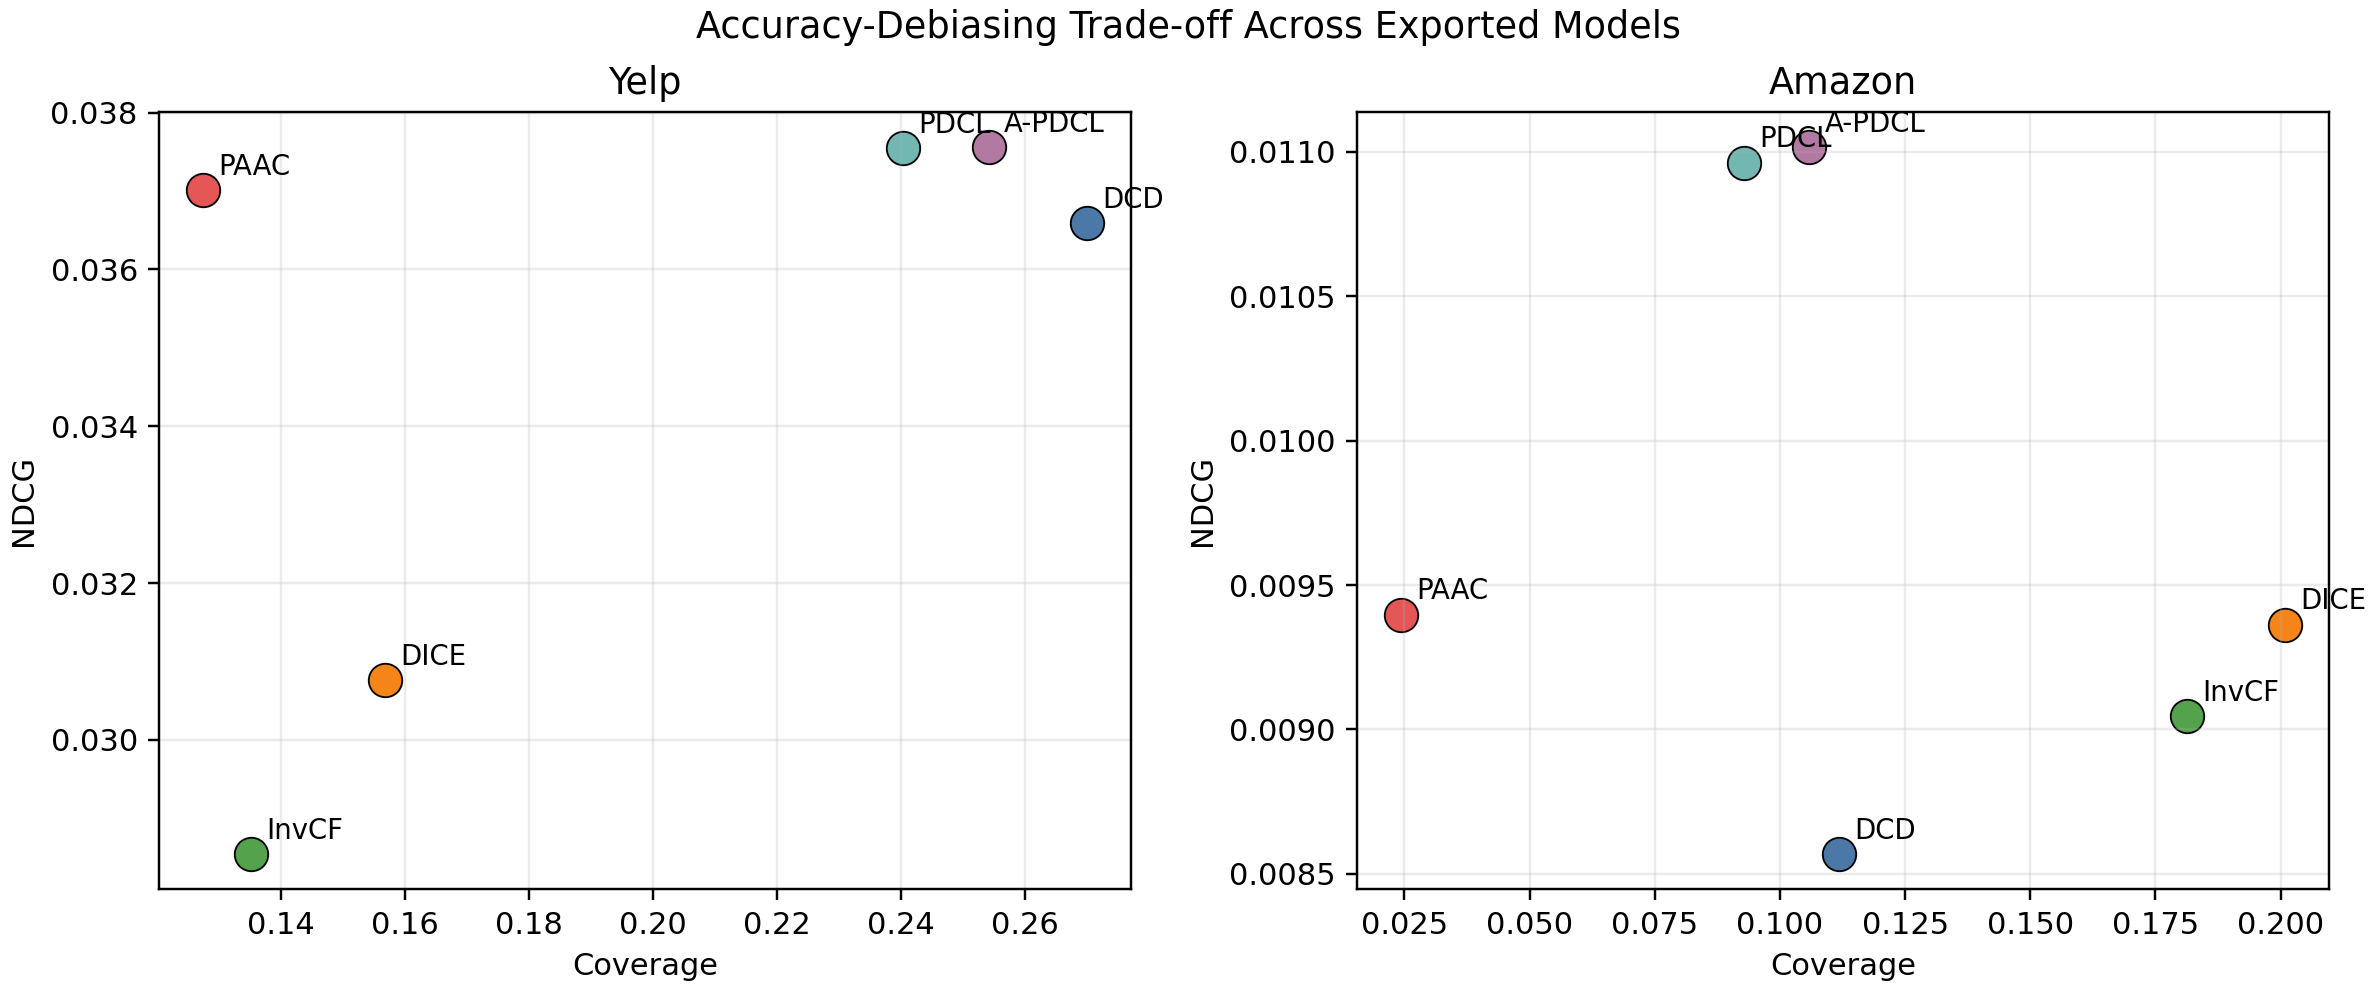
\includegraphics[width=0.9\textwidth]{fig_tradeoff_ndcg_coverage.png}
\caption{NDCG--coverage trade-off for the six recommendation models. Models close in NDCG but separated in coverage create the clearest test cases for debiasing sensitivity.}
\label{fig:tradeoff}
\end{figure}

On Yelp, DCD achieves the highest coverage (0.270) while PDCL and A-PDCL recover similar NDCG (0.0375--0.0376) with moderate coverage reduction. On Amazon, DICE has the broadest coverage (0.201) and InvCF the highest tail exposure (0.00172), while PDCL and A-PDCL achieve the best Recall and NDCG. These differences confirm that the benchmark compares meaningfully different systems rather than near-identical variants.

Critically, several pairs create diagnostic cases where accuracy and debiasing metrics point in opposite directions. For instance, A-PDCL achieves higher NDCG than DCD on both datasets but lower coverage on Yelp, creating a tension between relevance improvement and catalog diversity that an ideal judge should navigate. Similarly, InvCF vs.\ PAAC on Amazon presents a case where InvCF has substantially higher tail exposure (0.00172 vs.\ 0.00014) but lower NDCG (0.0090 vs.\ 0.0094), testing whether judges can detect debiasing gains that come at an accuracy cost. These deliberately constructed contrasts ensure that trivial alignment (e.g., always preferring the model with higher NDCG) does not produce perfect debiasing alignment.

\subsection{RQ1: Balanced prompts and metric alignment}

\subsubsection{Local judges}

Under the local phi-2 judge, balanced prompts fail to detect debiasing. Across all 20 pair-dimension records, the average bidirectional consistency is 0.957 (95\% CI [0.871, 1.000]), but this stability arises entirely from TIE saturation: the judge outputs TIE for every consistent trial. The resulting NDCG alignment is exactly 0.500 and coverage alignment is 0.500---indistinguishable from a random coin flip.

\begin{table}[t]
\centering
\caption{Average judge alignment and consistency for the local phi-2 benchmark run (seed 42). Alignment values of 0.5 indicate tie-dominated behavior.}
\label{tab:main_alignment}
\begin{tabular}{llccc}
\toprule
Dataset & Prompt & Align-NDCG & Align-Coverage & Consistency \\
\midrule
Amazon & Balanced & 0.500 & 0.500 & 1.000 \\
Amazon & Diversity & 0.500 & 0.500 & 1.000 \\
Amazon & Novelty & 0.500 & 0.500 & 0.976 \\
Amazon & Relevance & 0.400 & 0.400 & 0.524 \\
Yelp & Balanced & 0.500 & 0.500 & 0.940 \\
Yelp & Diversity & 0.500 & 0.500 & 1.000 \\
Yelp & Novelty & 0.500 & 0.500 & 0.936 \\
Yelp & Relevance & 0.500 & 0.500 & 0.944 \\
\midrule
\multicolumn{2}{l}{Overall average} & 0.487 & 0.487 & 0.915 \\
\bottomrule
\end{tabular}
\end{table}

The additional local judge, Qwen2.5-7B-Instruct (local), breaks the all-TIE failure mode but remains unreliable. Across the same 20 cross-judge records, it reaches only 0.262 bidirectional consistency (95\% CI [0.174, 0.362]), with 30\% aggregate ties, 0.450 NDCG alignment, and 0.600 coverage alignment. This is better calibrated to coverage than phi-2, but still far below the stability needed to serve as primary evidence for debiasing claims.

\subsubsection{Cloud judges}

Table~\ref{tab:consistency} reports the consistency statistics for all six judges. The four cloud judges still exhibit varied but uniformly problematic behaviors:

\begin{itemize}
\item \textbf{Qwen-Plus} expresses non-tie preferences in the vast majority of trials but achieves only 16.9\% bidirectional consistency (95\% CI [0.117, 0.223]). The 83.1\% inconsistency rate indicates severe position bias: verdicts flip when list order reverses.
\item \textbf{DeepSeek-V3} produces zero ties and achieves moderate consistency (54.2\%, 95\% CI [0.471, 0.605]). Its NDCG alignment and coverage alignment are both 60.0\%.
\item \textbf{Kimi-K2} achieves the highest consistency among cloud judges (66.0\%, 95\% CI [0.589, 0.728]) and the best coverage alignment (65.0\%).
\item \textbf{MiniMax-M2.7} shows intermediate consistency (46.0\%, 95\% CI [0.394, 0.526]) and the best NDCG alignment (65.0\%), but this apparent accuracy is not corroborated by broad cross-judge agreement.
\end{itemize}

\begin{table}[htbp]
\centering
\caption{Bidirectional consistency rate of each LLM judge across all pairwise comparisons.}
\label{tab:consistency}
\begin{tabular}{lcccc}
\hline
Judge & Mean & Std & 95\% CI & Range \\
\hline
Phi-2 (local) & 0.957 & 0.187 & [0.871, 1.000] & [0.14, 1.00] \\
Qwen2.5-7B-Instruct(local) & 0.262 & 0.207 & [0.174, 0.362] & [0.00, 0.84] \\
Qwen-Plus & 0.169 & 0.122 & [0.117, 0.223] & [0.00, 0.36] \\
DeepSeek-V3 & 0.542 & 0.150 & [0.471, 0.605] & [0.24, 0.76] \\
MiniMax-M2.7 & 0.460 & 0.152 & [0.394, 0.526] & [0.18, 0.70] \\
Kimi-K2 & 0.660 & 0.162 & [0.589, 0.728] & [0.34, 0.92] \\
\hline
\end{tabular}
\end{table}

\begin{figure}[t]
\centering
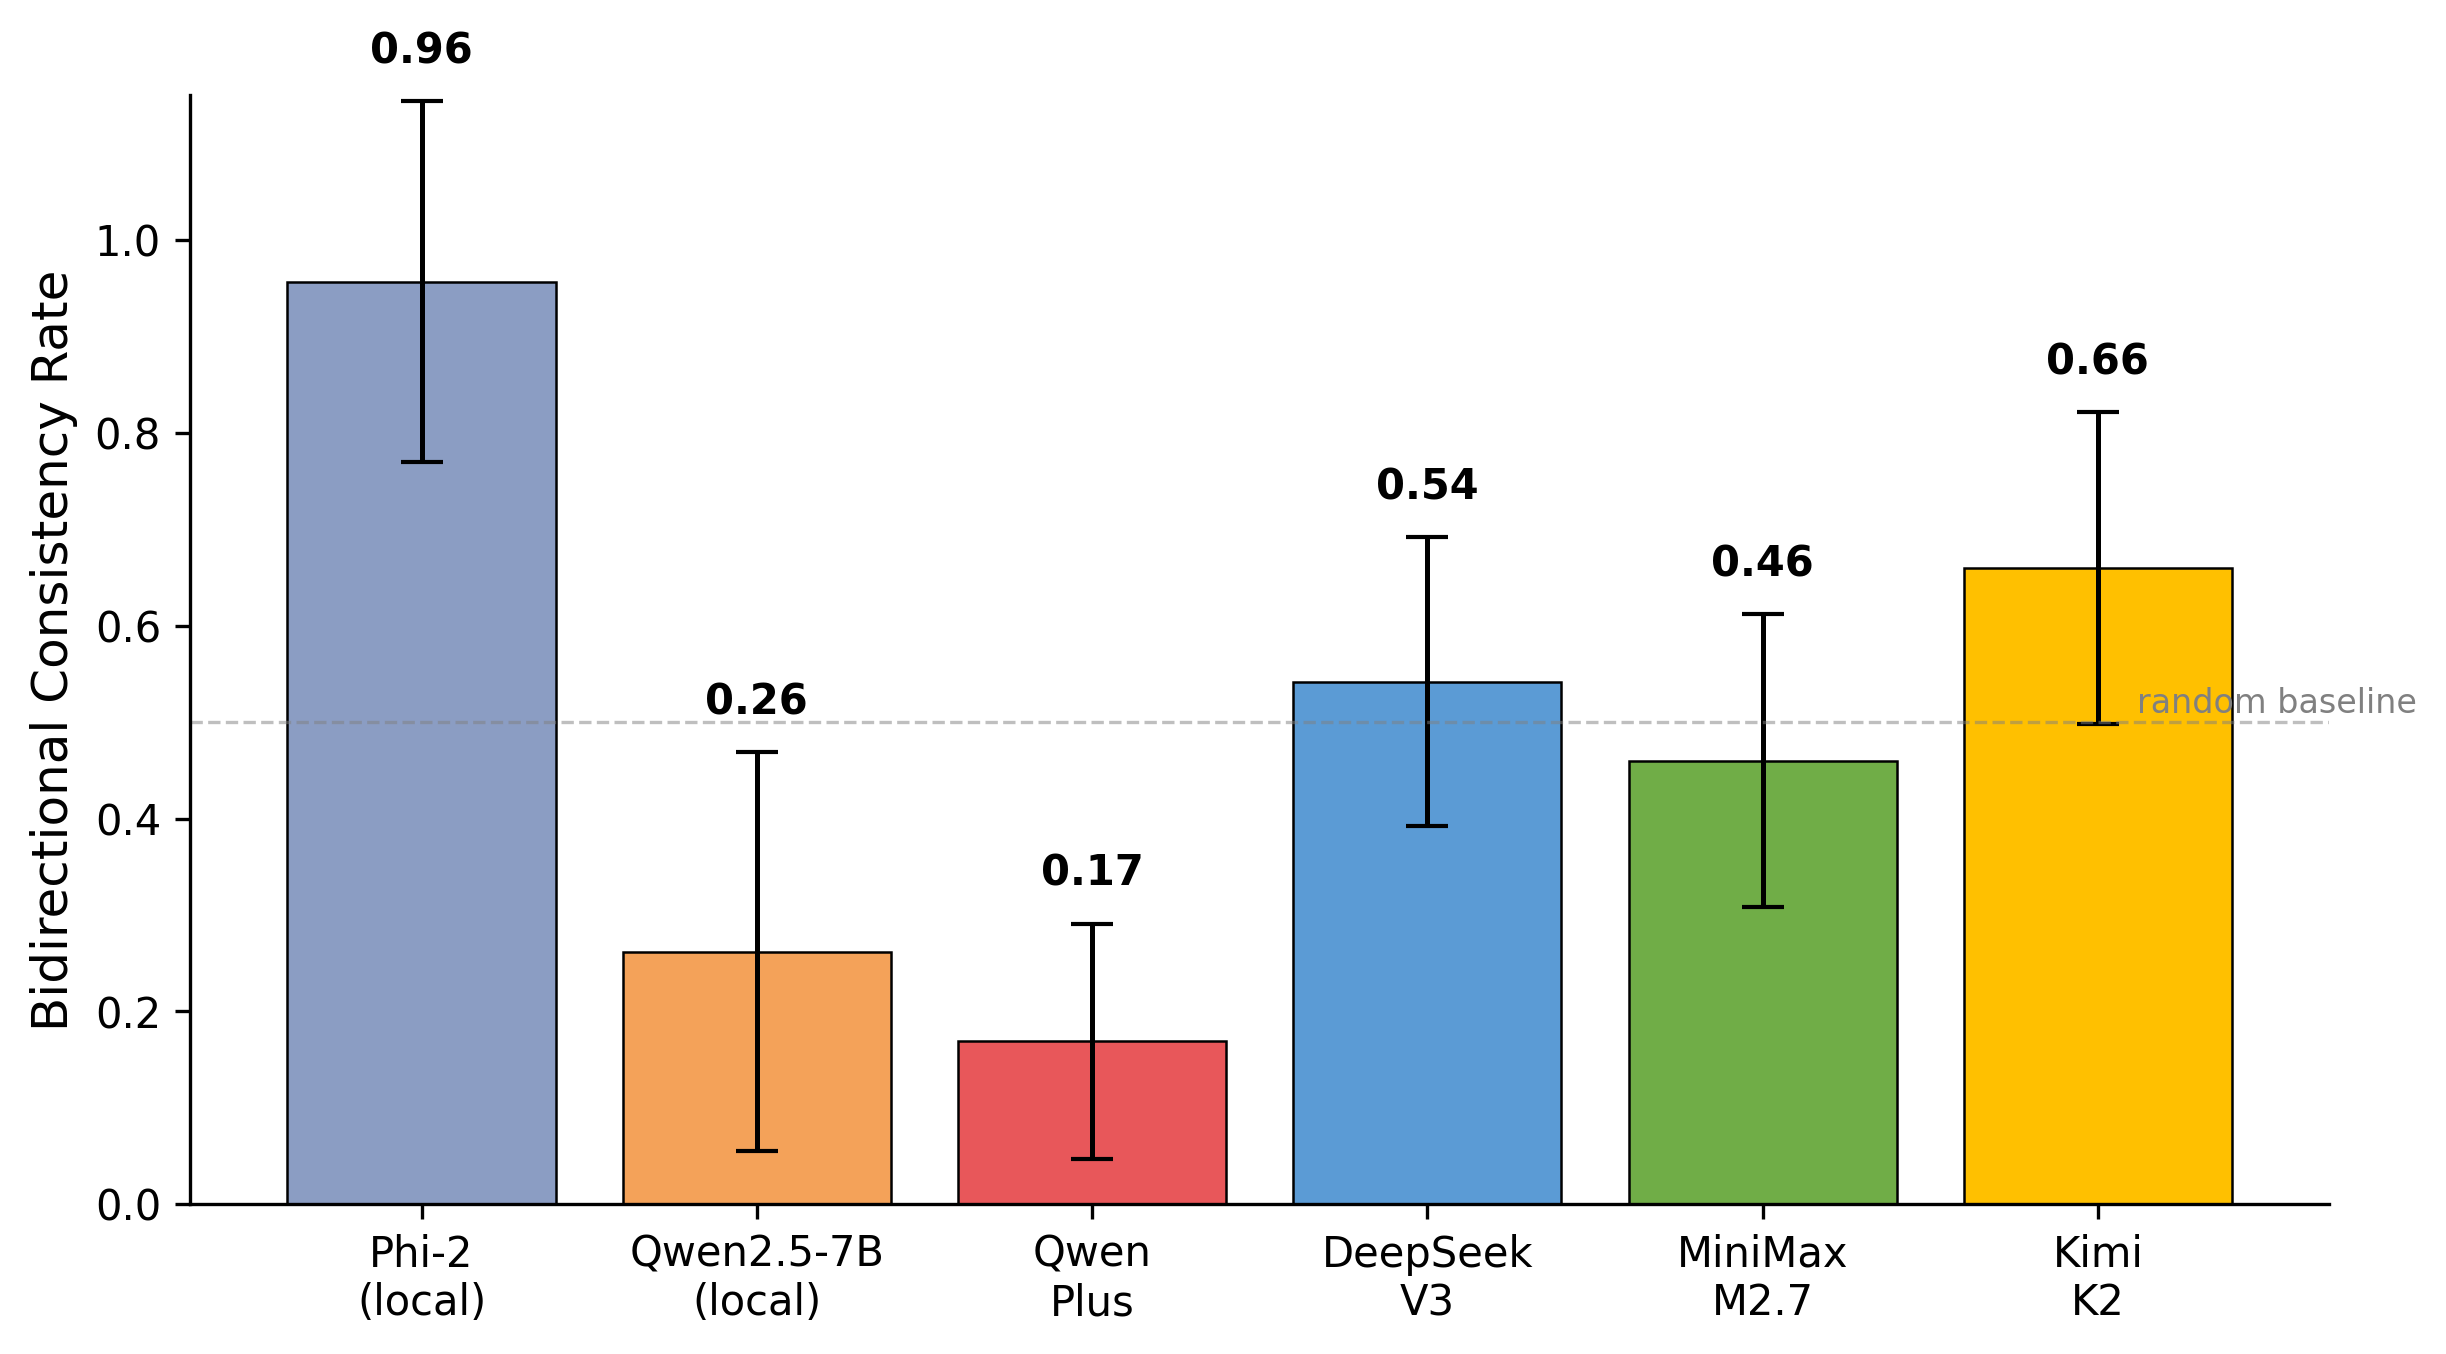
\includegraphics[width=0.95\columnwidth]{fig_consistency.png}
\caption{Bidirectional consistency rate across six LLM judges. Error bars indicate standard deviation. The dashed line marks the 0.5 random baseline. Phi-2 achieves near-perfect consistency through TIE saturation, while Qwen2.5-7B-Instruct (local) and the four cloud judges show varied but still unreliable discrimination.}
\label{fig:consistency}
\end{figure}

\subsection{RQ2: Prompt specialization}

Diversity prompts are the most plausible route for making judges notice long-tail improvements. However, under phi-2 both balanced and diversity prompts remain entirely tie-dominated. Across all six judges, balanced prompts yield slightly higher agreement than diversity prompts (Fleiss' $\kappa = 0.315$ vs.\ 0.298), and neither dimension pushes alignment above 0.65 for any judge. The improvement is insufficient to constitute reliable debiasing detection.

\begin{table*}[htbp]
\centering
\small
\caption{LLM judge verdicts across 6 judges for each debiasing pair comparison. Each cell shows the winner (A/B/tie) and bidirectional consistency rate in parentheses. Bold indicates agreement with NDCG ground truth.}
\label{tab:main-results}
\resizebox{\textwidth}{!}{%
\begin{tabular}{llllcccccc}
\hline
Dataset & Pair & Dim. & GT & Phi-2 & Qwen2.5-7B & Qwen-Plus & DeepSeek-V3 & MiniMax-M2.7 & Kimi-K2 \\
\hline
Yelp & dcd vs dice & bal & dcd & tie(100\%) & tie(4\%) & tie(16\%) & \textbf{dcd(76\%)} & tie(44\%) & \textbf{dcd(84\%)} \\
 &  & div & dcd & tie(100\%) & dice(18\%) & dice(32\%) & dice(64\%) & \textbf{dcd(18\%)} & dice(52\%) \\
 & dcd vs apdcl\_bmax10 & bal & apdcl\_bmax10 & tie(100\%) & tie(24\%) & \textbf{apdcl\_bmax10(2\%)} & \textbf{apdcl\_bmax10(50\%)} & \textbf{apdcl\_bmax10(42\%)} & \textbf{apdcl\_bmax10(58\%)} \\
 &  & div & apdcl\_bmax10 & tie(100\%) & tie(34\%) & dcd(12\%) & \textbf{apdcl\_bmax10(54\%)} & \textbf{apdcl\_bmax10(32\%)} & dcd(34\%) \\
 & dice vs apdcl\_bmax10 & bal & apdcl\_bmax10 & tie(100\%) & \textbf{apdcl\_bmax10(2\%)} & \textbf{apdcl\_bmax10(8\%)} & \textbf{apdcl\_bmax10(66\%)} & tie(36\%) & \textbf{apdcl\_bmax10(78\%)} \\
 &  & div & apdcl\_bmax10 & tie(100\%) & dice(12\%) & dice(24\%) & dice(74\%) & \textbf{apdcl\_bmax10(38\%)} & dice(62\%) \\
 & pdcl\_b05 vs apdcl\_bmax10 & bal & apdcl\_bmax10 & tie(100\%) & tie(8\%) & tie(0\%) & \textbf{apdcl\_bmax10(50\%)} & pdcl\_b05(56\%) & \textbf{apdcl\_bmax10(56\%)} \\
 &  & div & apdcl\_bmax10 & tie(100\%) & pdcl\_b05(16\%) & \textbf{apdcl\_bmax10(8\%)} & \textbf{apdcl\_bmax10(60\%)} & \textbf{apdcl\_bmax10(32\%)} & \textbf{apdcl\_bmax10(52\%)} \\
 & invcf vs paac & bal & paac & tie(100\%) & tie(0\%) & \textbf{paac(2\%)} & \textbf{paac(64\%)} & \textbf{paac(32\%)} & \textbf{paac(62\%)} \\
 &  & div & paac & tie(100\%) & invcf(14\%) & invcf(12\%) & invcf(58\%) & \textbf{paac(24\%)} & invcf(60\%) \\
\hline
Amazon & dcd vs dice & bal & dice & tie(100\%) & \textbf{dice(32\%)} & \textbf{dice(36\%)} & \textbf{dice(74\%)} & \textbf{dice(66\%)} & \textbf{dice(92\%)} \\
 &  & div & dice & tie(100\%) & \textbf{dice(22\%)} & tie(28\%) & dcd(48\%) & dcd(60\%) & dcd(76\%) \\
 & dcd vs apdcl\_bmax10 & bal & apdcl\_bmax10 & tie(100\%) & \textbf{apdcl\_bmax10(42\%)} & \textbf{apdcl\_bmax10(32\%)} & \textbf{apdcl\_bmax10(54\%)} & \textbf{apdcl\_bmax10(48\%)} & \textbf{apdcl\_bmax10(84\%)} \\
 &  & div & apdcl\_bmax10 & tie(100\%) & dcd(10\%) & tie(8\%) & dcd(28\%) & dcd(64\%) & dcd(78\%) \\
 & dice vs apdcl\_bmax10 & bal & apdcl\_bmax10 & tie(100\%) & \textbf{apdcl\_bmax10(42\%)} & dice(18\%) & \textbf{apdcl\_bmax10(56\%)} & \textbf{apdcl\_bmax10(44\%)} & \textbf{apdcl\_bmax10(80\%)} \\
 &  & div & apdcl\_bmax10 & tie(100\%) & dice(20\%) & dice(18\%) & dice(42\%) & dice(62\%) & dice(70\%) \\
 & pdcl\_b05 vs apdcl\_bmax10 & bal & apdcl\_bmax10 & tie(100\%) & \textbf{apdcl\_bmax10(84\%)} & tie(0\%) & \textbf{apdcl\_bmax10(24\%)} & \textbf{apdcl\_bmax10(32\%)} & \textbf{apdcl\_bmax10(50\%)} \\
 &  & div & apdcl\_bmax10 & tie(100\%) & tie(64\%) & \textbf{apdcl\_bmax10(12\%)} & \textbf{apdcl\_bmax10(24\%)} & \textbf{apdcl\_bmax10(52\%)} & \textbf{apdcl\_bmax10(34\%)} \\
 & invcf vs paac & bal & paac & tie(100\%) & invcf(38\%) & invcf(36\%) & invcf(64\%) & invcf(68\%) & invcf(84\%) \\
 &  & div & paac & tie(14\%) & invcf(38\%) & invcf(34\%) & invcf(54\%) & invcf(70\%) & invcf(74\%) \\
\hline
\end{tabular}%
}
\end{table*}

Table~\ref{tab:main-results} presents the full verdict matrix across all six judges. Several patterns emerge: (i) A-PDCL is most frequently selected as the winner under balanced prompts, consistent with its strong NDCG performance; (ii) diversity prompts increase disagreement among judges, with some reversing their preferences; (iii) the InvCF--PAAC pair produces the most inconsistent judgments, possibly because these models differ primarily in distributional rather than textual properties.

\subsection{RQ3: Description normalization}

The title-only condition strips item descriptions to compact representations, reducing each item from potentially multi-sentence descriptions (especially in Amazon, where product descriptions average 50--100 words) to a single title string. The motivation is to test whether verbose descriptions introduce a text-richness confound: judges might prefer lists whose items happen to have longer, more detailed descriptions rather than lists that genuinely serve the user better.

Across all 20 DescNorm records with the local judge, the outcome is unchanged: 100\% TIE, 1.0 consistency, 0.5 alignment. Removing textual richness does not recover debiasing sensitivity; the failure mode is robust to presentation simplification. This result rules out an optimistic hypothesis---that Phi-2's tie saturation stems from information overload rather than fundamental incapacity. Even with dramatically simplified inputs, the local judge cannot engage with the comparison task.

For a complete picture of DescNorm effects on cloud judges, we additionally evaluate DeepSeek-V3 under the title-only condition. This serves as a controlled test of whether the most discriminative cloud judge changes behavior when textual richness is reduced. Results for this extension are discussed in Section~\ref{sec:discussion}.

\subsection{RQ4: Cross-judge analysis}

\subsubsection{Inter-judge agreement}

Table~\ref{tab:kappa} presents pairwise Cohen's $\kappa$ between all judges, and Table~\ref{tab:fleiss} reports Fleiss' $\kappa$ for multi-rater agreement. The key findings are:

\begin{enumerate}
\item \textbf{A partial cluster structure emerges.} DeepSeek-V3 and Kimi-K2 remain the strongest-agreement pair ($\kappa = 0.931$). Qwen2.5-7B-Instruct (local) shows moderate agreement with both ($\kappa = 0.518$ and $0.522$), while Phi-2 remains isolated at $\kappa = 0.000$ because of its all-TIE behavior.
\item \textbf{Overall agreement is fair but not reliable.} Fleiss' $\kappa = 0.326$ across all six judges indicates fair agreement beyond chance but far below the $\kappa > 0.6$ threshold typically required for substantive agreement \citep{fleiss1971kappa}.
\item \textbf{Agreement varies by dimension and dataset.} Balanced prompts yield slightly higher agreement ($\kappa = 0.315$) than diversity prompts ($\kappa = 0.298$). Amazon produces substantially higher agreement ($\kappa = 0.413$) than Yelp ($\kappa = 0.224$).
\end{enumerate}

\begin{table}[htbp]
\centering
\caption{Pairwise Cohen's $\kappa$ between LLM judges on winner labels.}
\label{tab:kappa}
\scriptsize
\setlength{\tabcolsep}{2pt}
\begin{tabular}{lcccccc}
\hline
 & Phi-2 & Qwen2.5-7B & Qwen-Plus & DeepSeek-V3 & MiniMax-M2.7 & Kimi-K2 \\
\hline
Phi-2 & 1.000 & 0.000 & 0.000 & 0.000 & 0.000 & 0.000 \\
Qwen2.5-7B & 0.000 & 1.000 & 0.429 & 0.518 & 0.345 & 0.522 \\
Qwen-Plus & 0.000 & 0.429 & 1.000 & 0.565 & 0.392 & 0.632 \\
DeepSeek-V3 & 0.000 & 0.518 & 0.565 & 1.000 & 0.604 & 0.931 \\
MiniMax-M2.7 & 0.000 & 0.345 & 0.392 & 0.604 & 1.000 & 0.545 \\
Kimi-K2 & 0.000 & 0.522 & 0.632 & 0.931 & 0.545 & 1.000 \\
\hline
\end{tabular}
\end{table}
\begin{table}[htbp]
\centering
\caption{Fleiss' $\kappa$ measuring agreement among all 6 LLM judges.}
\label{tab:fleiss}
\begin{tabular}{lc}
\hline
Scope & Fleiss' $\kappa$ \\
\hline
Overall & 0.3255 \\
Balanced & 0.3151 \\
Diversity & 0.2975 \\
Yelp & 0.2244 \\
Amazon & 0.4132 \\
\hline
\end{tabular}
\end{table}

\begin{figure}[t]
\centering
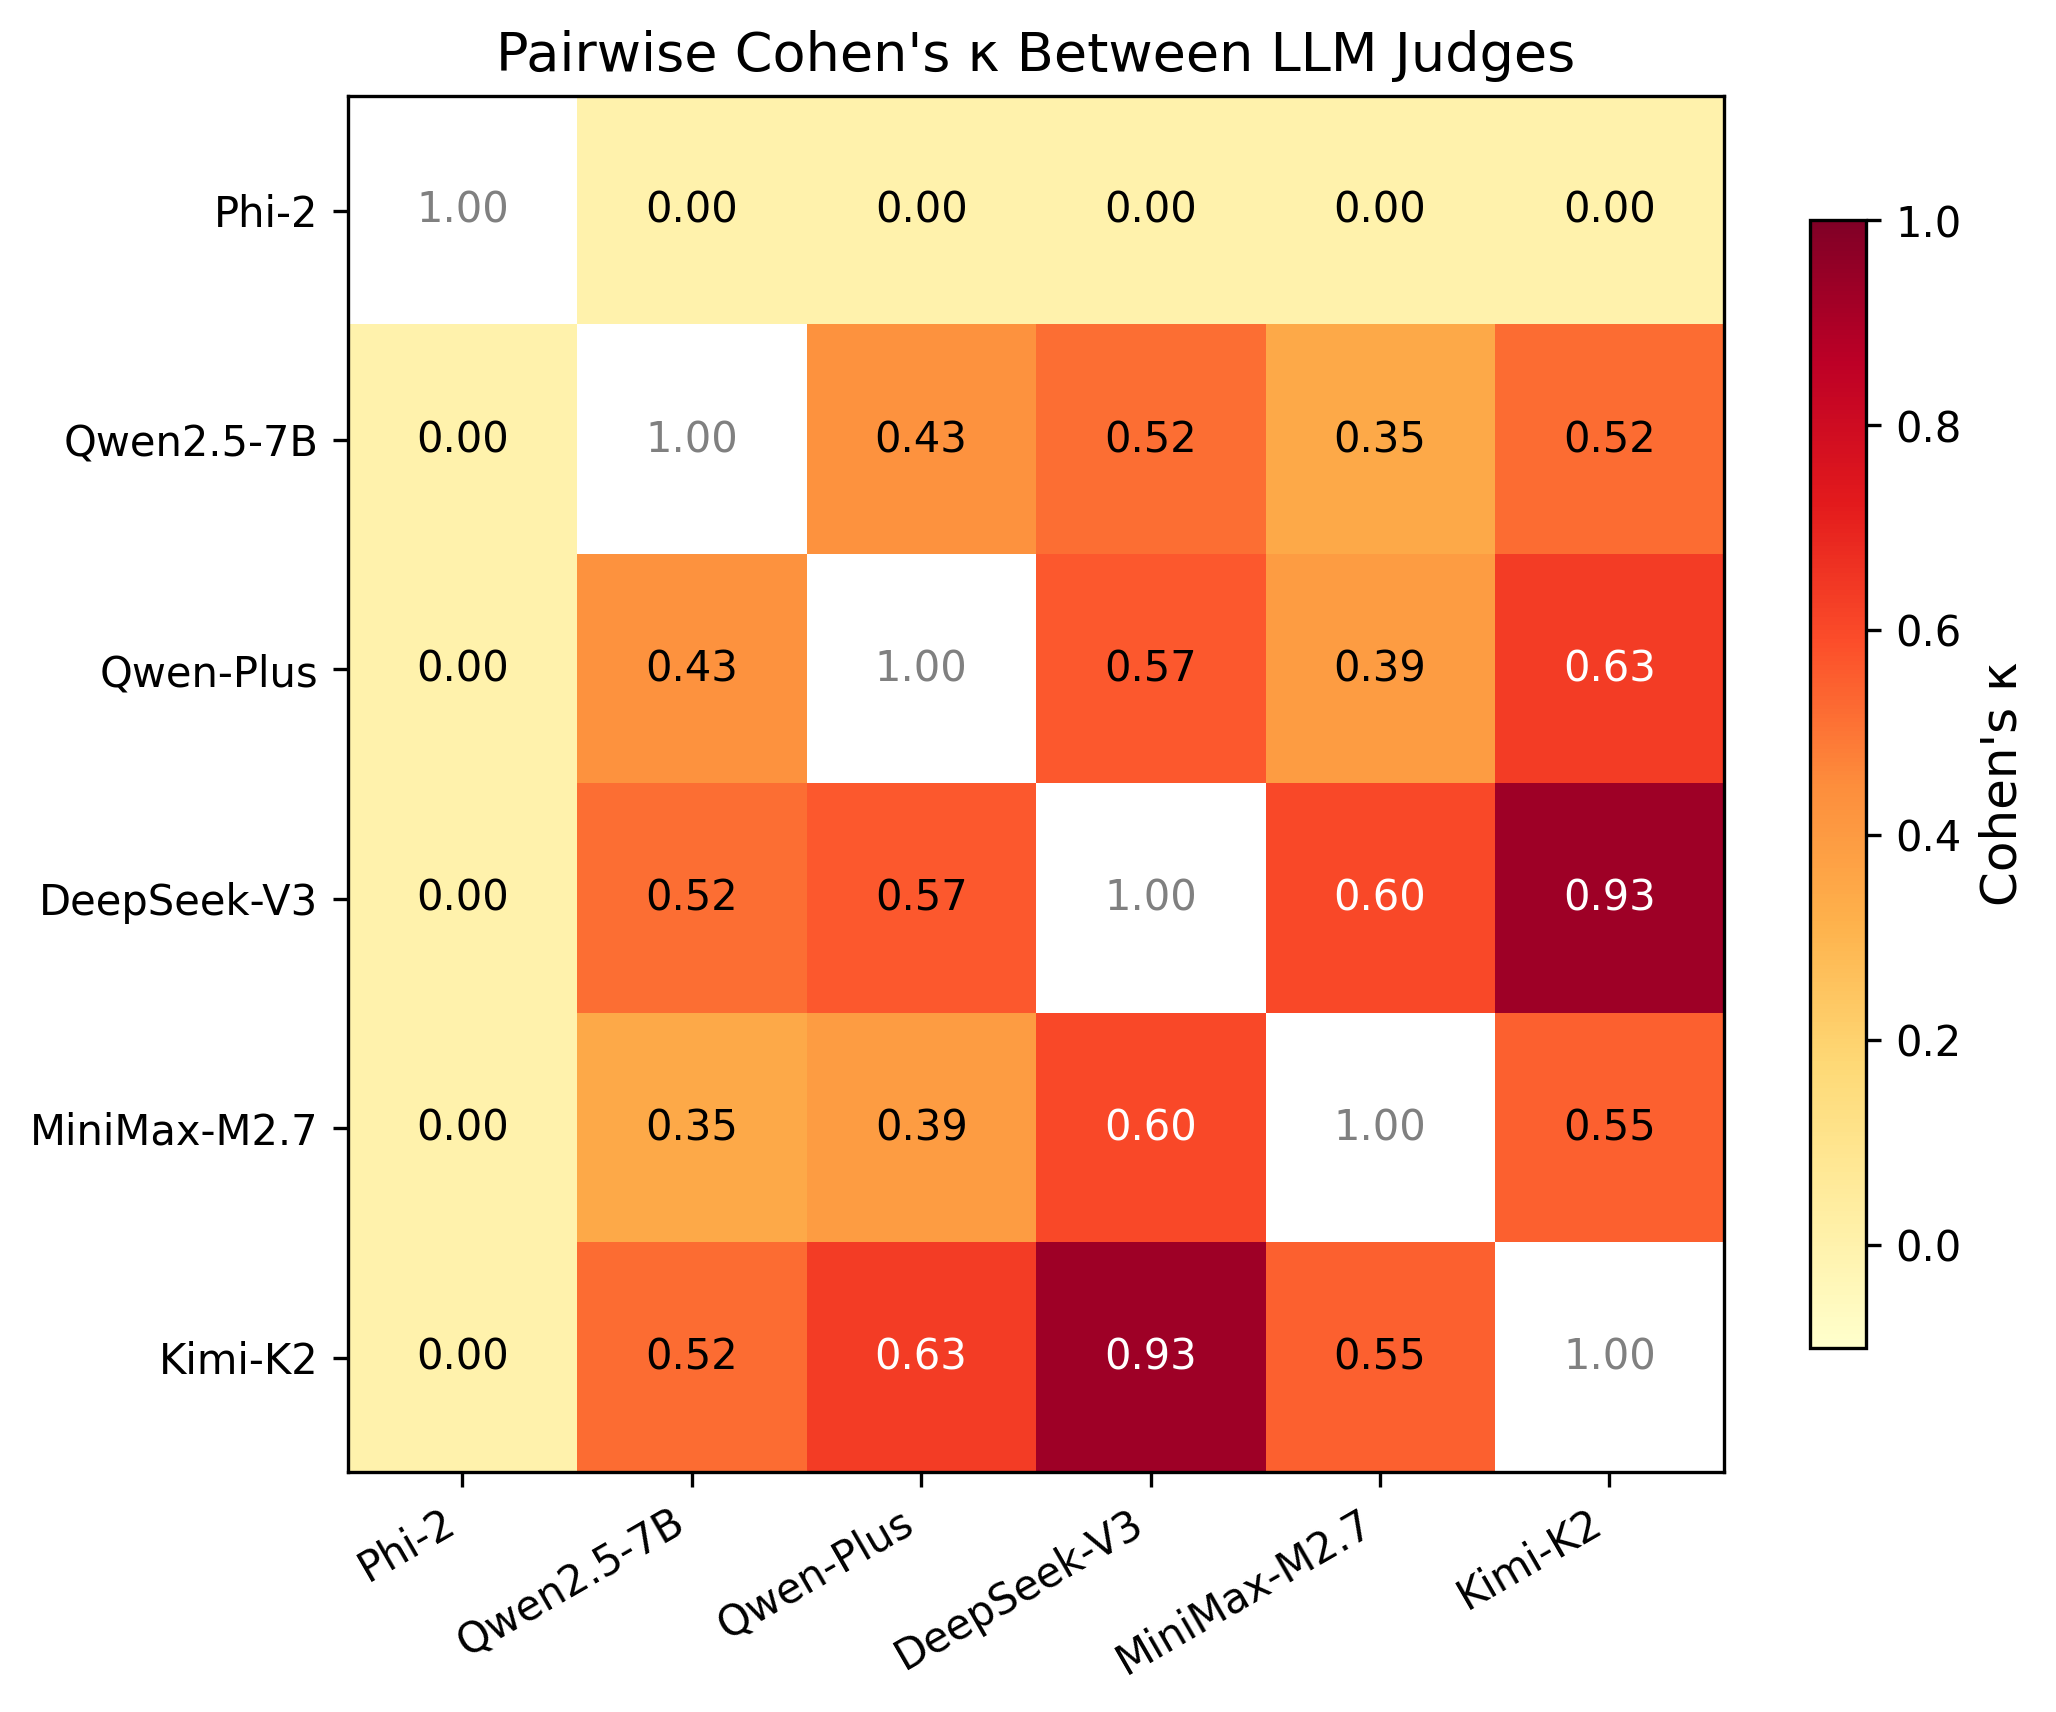
\includegraphics[width=0.85\columnwidth]{fig_kappa_heatmap.png}
\caption{Heatmap of pairwise Cohen's $\kappa$ between LLM judges. DeepSeek-V3 and Kimi-K2 show near-perfect agreement ($\kappa = 0.931$), Qwen2.5-7B-Instruct (local) shows only moderate agreement with that pair, and Phi-2 remains isolated by all-TIE behavior.}
\label{fig:kappa_heatmap}
\end{figure}

\subsubsection{Alignment to ground-truth metrics}

Figure~\ref{fig:alignment} compares the fraction of experiment pairs where each judge's verdict matches the NDCG-based or coverage-based ground truth.

\begin{figure}[t]
\centering
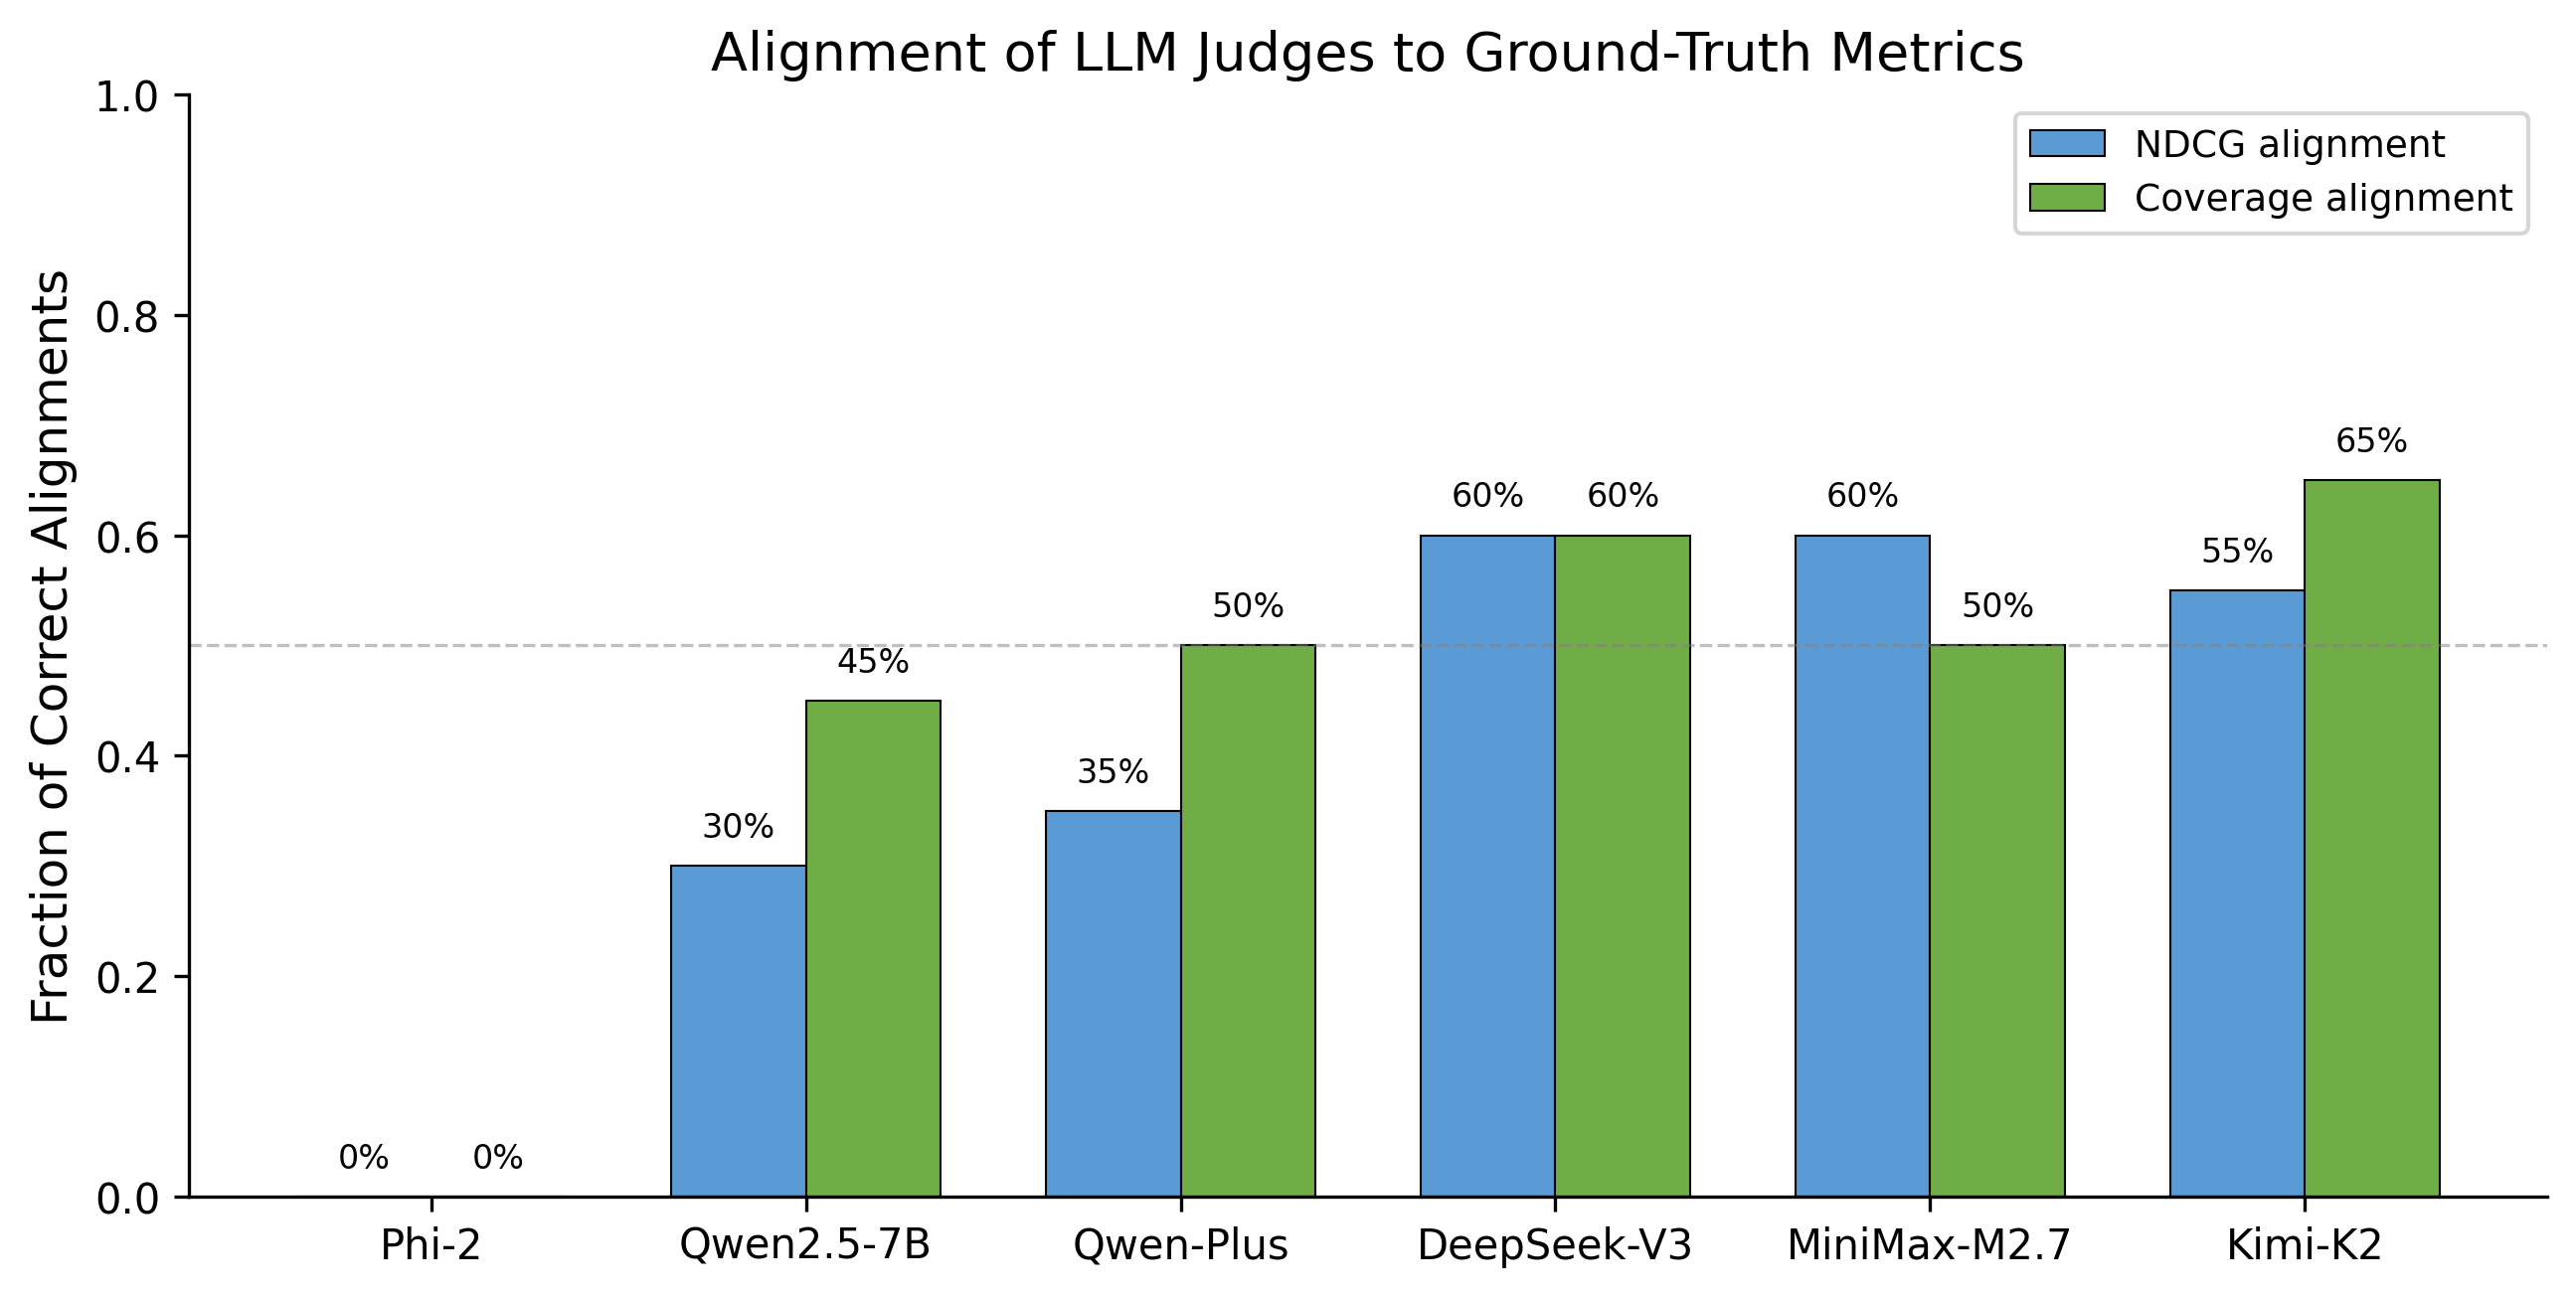
\includegraphics[width=0.95\columnwidth]{fig_alignment.png}
\caption{Alignment of LLM judge verdicts to ground-truth offline metrics. No judge exceeds 65\% alignment on either metric, and Phi-2's alignment is exactly 50\% (random chance) due to tie saturation.}
\label{fig:alignment}
\end{figure}

\subsubsection{Rank correlation}

Most Spearman rank correlations between judges' consistency-rate vectors are non-significant. The significant pairs are Qwen2.5-7B-Instruct (local) vs.\ DeepSeek-V3 ($\rho = -0.455$, $p = 0.044$), Qwen-Plus vs.\ MiniMax-M2.7 ($\rho = 0.450$, $p = 0.047$), Qwen-Plus vs.\ Kimi-K2 ($\rho = 0.543$, $p = 0.013$), and MiniMax-M2.7 vs.\ Kimi-K2 ($\rho = 0.568$, $p = 0.009$). The mixed signs and sparse significance confirm that different judge architectures perceive pair difficulty differently.

\subsubsection{Summary of cross-judge findings}

Three failure archetypes persist across all six judges:
\begin{itemize}
\item \emph{Tie saturation} (Phi-2): 95.7\% consistency through non-commitment, zero discriminative power.
\item \emph{Position bias} (Qwen-Plus): strong preferences driven by list position (83.1\% inconsistency).
\item \emph{Weak-to-moderate discrimination without reliable convergence} (Qwen2.5-7B-Instruct (local), DeepSeek-V3, MiniMax-M2.7, Kimi-K2): these judges avoid pure tie saturation but still yield unstable or only partially corroborated verdicts.
\end{itemize}
Under blind local pairwise judging without popularity metadata, moving from 2.7B to 671B parameters and from local to cloud inference changes the failure mode but does not produce reliable debiasing detection.

\subsection{Human sanity check}

To test whether the benchmark failure is unique to LLM judges, we analyzed the human sanity check described in Section~\ref{sec:human_sanity}. The result is stark: inter-rater agreement is effectively absent (Fleiss' $\kappa = 0.005$) even though mean duplicate consistency under list reversal reaches 76.7\%. Across the 40 base tasks, only 7 receive unanimous judgments, 26 end in a 2:1 split, and 7 produce three different verdicts.

Using the same 1.0/0.5/0.0 task-level alignment score as in the LLM analysis and averaging over the 40 base tasks, the human majority verdict reaches only 11.3\% alignment to the offline NDCG winner and 11.3\% alignment to the coverage winner. This is far below even a minimally useful evaluation threshold. The pattern suggests that annotators are not behaving randomly, but they are relying on incompatible local heuristics when the task is framed as a blind pairwise comparison without popularity cues. In other words, the central failure is not limited to LLMs: the local evaluation task itself under-exposes the distributional signal that debiasing methods are designed to improve.

\subsection{Popularity-aware validation probe}

The constructive probe materially changes the interpretation of the benchmark. On Qwen2.5-7B-Instruct (local), explicit popularity cues raise average consistency from 0.262 to 0.550 and improve alignment to coverage (0.600$\rightarrow$0.650), Gini (0.550$\rightarrow$0.750), and ARP (0.550$\rightarrow$0.700), while tail-exposure alignment remains flat overall. The gains are uneven: balanced comparisons benefit more than diversity, and diversity still exhibits local regressions on coverage and tail exposure.

For DeepSeek-V3, the effect is stronger. Consistency rises from 0.542 to 0.810, coverage and tail-exposure alignment each improve from 0.600 to 0.750, and Gini/ARP alignment rise from 0.600 to 0.850. Unlike the local 7B judge, DeepSeek-V3 also improves sharply on diversity prompts, where consistency gains reach +0.454 and tail-exposure alignment gains reach +0.300. The main trade-off is NDCG: for DeepSeek-V3 it drops from 0.600 to 0.550 overall, with a pronounced balanced-prompt drop from 0.900 to 0.500.

These results refine the core claim of the paper. The blind protocol does not merely reveal weak judges; it actively hides the distributional evidence that debiasing methods are designed to improve. Once popularity metadata is made explicit, at least some judges recover substantial sensitivity, although not enough to displace offline metrics as the primary evidence for long-tail claims.

%% ============================================================
\section{Discussion}
\label{sec:discussion}
%% ============================================================

\subsection{A taxonomy of LLM judge failures for debiasing}

The central finding is two-part. Under blind local pairwise judging, six qualitatively different LLM judges fail to reliably detect popularity debiasing, but through distinct mechanisms. However, a simple popularity-aware prompt partially restores sensitivity for two judges, especially DeepSeek-V3. The limitation is therefore best understood as protocol-level rather than purely model-level.

\noindent\textbf{Tie saturation.}  The smallest judge (phi-2, 2.7B) lacks the discriminative capacity to distinguish between recommendation lists that differ primarily in catalog-level properties. Its 100\% TIE rate among consistent trials produces 0.500 alignment to any metric by construction. This archetype is likely to affect any judge whose language modeling capability is insufficient to resolve subtle quality differences in long item descriptions.

\noindent\textbf{Position bias.}  Larger judges (especially Qwen-Plus) have sufficient capability to express preferences but apply that capability to surface features---principally which list appears first---rather than to content quality. With only 16.9\% bidirectional consistency, Qwen-Plus reverses its verdict 83.1\% of the time when list order is swapped. This finding is consistent with prior work showing that position bias in pairwise LLM evaluation can be systematic rather than random \citep{raina2025judging}, but we extend it to a new domain (recommendation debiasing) where the consequence is particularly severe: a position-biased judge produces unstable and unreliable alignment with any offline metric.

\noindent\textbf{Weak-to-moderate discrimination with partial convergence.}  Qwen2.5-7B-Instruct (local), DeepSeek-V3, MiniMax-M2.7, and Kimi-K2 partially avoid both extremes, but with very different reliability. Qwen2.5-7B-Instruct (local) breaks phi-2's all-TIE regime yet reaches only 26.2\% consistency, indicating weak local discrimination rather than robust judgment. DeepSeek-V3, MiniMax-M2.7, and Kimi-K2 produce more decisive preferences at 54.2\%, 46.0\%, and 66.0\%, respectively. DeepSeek-V3 and Kimi-K2 also achieve near-perfect mutual agreement ($\kappa = 0.931$). However, this convergence does not extend to the full panel: Qwen2.5-7B-Instruct (local) reaches only moderate agreement with the stronger cluster ($\kappa = 0.518$ with DeepSeek-V3 and $0.522$ with Kimi-K2), while MiniMax-M2.7 remains idiosyncratic despite its 65.0\% NDCG alignment. None of these judges exceeds 65\% alignment on either offline metric, so decisiveness does not translate into reliable debiasing detection.

\subsection{Why blind local judging hides debiasing signals}

The fundamental mismatch is between the \emph{level of analysis}. Coverage, Gini, ARP, and tail exposure are population-level statistics: they describe how recommendations are distributed across the item catalog for all users. A blind pairwise LLM judge sees a single user's two lists, each containing 10--20 items from a catalog of tens or hundreds of thousands. Without explicit popularity metadata, the judge cannot directly observe whether the items in list B are more ``long-tail'' than those in list A.

The popularity-aware probe makes this causal story harder to dismiss. Once HEAD/MID/TAIL evidence is exposed, Qwen2.5-7B-Instruct (local) becomes materially more stable and DeepSeek-V3 becomes substantially more aligned with coverage, tail exposure, Gini, and ARP. The blind protocol is therefore not a neutral presentation choice; it suppresses the very signal that a debiasing-sensitive judge would need to use.

This does not mean that distributional debiasing becomes trivial once metadata is added. Even a hypothetically perfect text-understanding model must still balance semantic relevance against population-level diversity and long-tail exposure. The constructive result instead shows that the original blind setup is under-specified for this task \citep{mcnee2006being,herlocker2004evaluating}.

\subsection{Human raters face the same blind spot}

The human sanity check rules out an overly simple explanation that the benchmark fails only because current LLMs are poor evaluators. Under the same blind local pairwise setup, three human annotators reach only Fleiss' $\kappa = 0.005$ and 11.3\% alignment to either offline winner, despite moderate self-consistency under reversed duplicates (76.7\%). Humans therefore exhibit some intra-rater stability without reaching a shared decision criterion.

This matters for interpretation. If both humans and LLM judges fail under the same protocol, then the main problem is not merely model scale, instruction-following quality, or provider-specific bias. The deeper issue is that a single user's two textual lists do not reveal enough information about coverage, catalog concentration, or tail exposure for reliable judgment. Without explicit popularity metadata or aggregated system-level evidence, blind local pairwise comparison is an under-specified instrument for evaluating distributional debiasing.

\subsection{Explicit popularity cues partially restore sensitivity}

Our constructive probe matters because it breaks the pure negative-result framing. The local 7B judge becomes markedly more stable, and DeepSeek-V3 becomes substantially more aligned with the distributional metrics that matter for debiasing once popularity evidence is made explicit. This is exactly what we would expect if the blind protocol suppresses the target signal rather than if LLM judges were fundamentally incapable of distributional reasoning.

At the same time, the recovery is incomplete. DeepSeek-V3 loses some NDCG alignment under the popularity-aware prompt, and the local 7B judge still struggles on diversity-sensitive cases. Explicit metadata therefore changes the trade-off rather than solving evaluation outright. This is why offline metrics remain primary evidence: the prompt can redirect attention toward distributional properties, but it does not guarantee calibrated multi-objective reasoning.

\subsection{Implications for evaluation practice}

Our findings do not argue that LLM judges should be abandoned. Rather, they prescribe specific safeguards:

\begin{enumerate}
\item \textbf{Retain offline debiasing metrics as primary evidence.} Coverage, Gini, ARP, and tail exposure should remain the foundation for long-tail claims. LLM judges are not reliable substitutes.
\item \textbf{Always include bidirectional evaluation.} Any LLM-based recommendation comparison should report consistency rates. A judge with $<50\%$ consistency is dominated by position effects and its aggregate preferences are unreliable.
\item \textbf{Report inter-judge agreement.} Single-judge evaluation hides model-specific biases. Cross-judge protocols with agreement statistics (Fleiss' $\kappa$, pairwise Cohen's $\kappa$) reveal whether findings are robust.
\item \textbf{Validate judge sensitivity before deployment.} If a judge cannot detect known metric differences in controlled comparisons, it should not be trusted for novel evaluation claims.
\end{enumerate}

A practical implication is that blind local pairwise judging should not be used as the sole evidence for debiasing claims when any of the following conditions hold:

\begin{itemize}
\item the target quality dimension is fundamentally distributional (for example, coverage, concentration, or tail exposure);
\item the judge sees only one user and two lists, without explicit popularity metadata or aggregated catalog statistics;
\item bidirectional consistency, human agreement, or cross-judge agreement remains low on controlled calibration cases.
\end{itemize}

Under these conditions, the safer evaluation design is hybrid: use offline distributional metrics for debiasing claims, and reserve human or LLM judgments for supplementary semantic criteria such as relevance, coherence, and perceived usefulness.

\subsection{Connection to broader LLM evaluation challenges}

Our negative findings resonate with broader concerns about LLM-based evaluation. \citet{shen2023large} showed that LLMs are not yet human-level evaluators for abstractive summarization; \citet{chen2024humans} documented systematic judgment biases in human-vs-LLM evaluation comparisons. The non-transitivity problem identified by \citet{liu2025nontransitivity} suggests that even if individual pairwise comparisons were reliable, aggregating them into rankings would introduce additional distortions.

Our work extends these concerns to a specific, high-stakes application: when the target quality dimension is distributional rather than textual, blind local LLM judging faces a structural disadvantage that model scaling alone does not address. The popularity-aware probe shows that part of this disadvantage is recoverable when the protocol exposes the right evidence, but the recovery is still incomplete. This observation has implications beyond recommendation. Any evaluation task where quality is defined at the population level---fairness auditing, diversity assessment, calibration testing---may exhibit the same mismatch between local textual judgment and global distributional properties unless the protocol surfaces the relevant aggregate signal.

The strongest cluster we observe is DeepSeek-V3 and Kimi-K2, with the added Qwen2.5-7B-Instruct (local) judge only partially approaching that pair. This pattern echoes findings in multi-annotator studies where annotators cluster by implicit evaluation criteria \citep{fleiss1971kappa}. The high pairwise agreement within the strongest cluster ($\kappa = 0.931$), combined with only fair overall agreement (Fleiss' $\kappa = 0.326$), suggests that different LLM architectures may attend to fundamentally different textual features when comparing recommendation lists. Understanding what features drive each judge's decisions---through attention analysis, feature attribution, or probing experiments---is an important direction for improving judge reliability.

\subsection{Future directions}

Our negative findings naturally suggest several avenues for future work aimed at closing the gap between LLM judgment and distributional debiasing metrics:

\noindent\textbf{Popularity-aware prompting.}  Our results already show that explicit popularity metadata can partially recover sensitivity, but only in a coarse form (HEAD/MID/TAIL labels and short list-level summaries) and only for two judges. Future work should test richer metadata designs---for example popularity percentiles, historical interaction counts, or calibrated long-tail annotations---and measure whether they can improve distributional alignment without sacrificing relevance-sensitive behavior.

\noindent\textbf{Aggregated judging protocols.}  Since debiasing is a population-level phenomenon, a natural extension is to provide judges with \emph{aggregated} information rather than single-user comparisons. For example, a judge could be shown summary statistics across $k$ users, such as the number of unique items recommended by each system across 50 users, and then asked to evaluate catalog diversity. This moves closer to how human evaluators assess debiasing in practice and may better align with distributional metrics.

\noindent\textbf{Fine-tuned evaluation models.}  Domain-specific fine-tuning on recommendation evaluation tasks, potentially using human judgments about recommendation diversity as training signal, could produce specialized judges that attend to the long-tail properties that general-purpose LLMs miss. The benchmark introduced here provides a natural test bed for such fine-tuned evaluators.

\noindent\textbf{Hybrid evaluation frameworks.}  Rather than replacing offline metrics with LLM judges, a more promising approach may combine both: use offline metrics for distributional claims and LLM judges for semantic quality assessment. Developing principled frameworks for integrating these complementary signals is an important direction for the recommendation evaluation community.

\subsection{Limitations}

Several scope conditions apply. First, the six blind judges cover five model families but not all major architectures (e.g., GPT-4o, Claude, Gemini). The inclusion of additional frontier models could reveal whether some architectures are inherently better suited to distributional reasoning. Second, the popularity-aware probe is currently limited to two judges---Qwen2.5-7B-Instruct (local) and DeepSeek-V3---and uses only coarse HEAD/MID/TAIL annotations plus short list-level summaries. Stronger judges, richer popularity metadata, or alternative prompt scaffolds may produce different recovery patterns. Third, the 50-user sample per pair, while sufficient for detecting large effects and establishing bidirectional consistency patterns, limits statistical power for detecting subtle alignment differences between judges. Fourth, the human sanity check is intentionally small-scale: it involves three annotators and 40 base tasks, and is designed as a diagnostic probe rather than a population-level estimate of human evaluation quality. Fifth, we evaluate pairwise comparison only; pointwise or listwise evaluation protocols may behave differently, and listwise protocols in particular could better capture distributional properties. Sixth, the debiasing models all share a LightGCN backbone; testing with architecturally diverse recommendation models would strengthen generalizability claims. These caveats define the boundary of the current benchmark and the current constructive probe without weakening the core contribution.

%% ============================================================
\section{Conclusion}
\label{sec:conclusion}
%% ============================================================

This paper introduces and validates a multi-judge evaluation protocol, instantiated as a benchmark, for testing whether LLM judges can detect popularity debiasing in recommender systems. By pairing six trained debiasing models on two datasets with six LLM judges spanning 2.7B to 671B parameters across five model families, we show that blind local pairwise judging is a poor instrument for distributional debiasing evaluation: under the blind protocol, no tested judge reliably aligns with offline metrics (best alignment: 65.0\%), and even human annotators fail to recover a stable criterion.

Three failure archetypes emerge under the blind protocol---tie saturation (Phi-2, 95.7\% consistency but zero discrimination), position bias (Qwen-Plus, 83.1\% verdict reversal), and weak-to-moderate discrimination without reliable metric alignment (Qwen2.5-7B-Instruct (local), DeepSeek-V3, MiniMax-M2.7, and Kimi-K2). Prompt specialization and description normalization do not recover sensitivity, and overall inter-judge agreement remains fair at best (Fleiss' $\kappa = 0.326$). The human sanity check reaches Fleiss' $\kappa = 0.005$ and only 11.3\% alignment to the offline winner, indicating that the blind task itself is under-specified for distributional debiasing.

A constructive extension changes the interpretation. When we expose explicit popularity evidence through per-item HEAD/MID/TAIL labels and list-level popularity summaries, Qwen2.5-7B-Instruct (local) improves from 0.262 to 0.550 consistency and DeepSeek-V3 improves from 0.542 to 0.810 consistency, with DeepSeek-V3 raising both coverage and tail-exposure alignment from 0.600 to 0.750. The main bottleneck is therefore not simply model scale; it is a protocol that hides the debiasing signal from the judge.

The practical message is clear. Offline distributional metrics such as coverage, Gini concentration, ARP, and tail exposure should remain the primary basis for long-tail claims. Blind local pairwise LLM judging should not be used as sole evidence for distributional improvement. LLM judges remain useful as supplementary semantic evaluators, and they become more informative when their sensitivity is explicitly validated or when the prompt surfaces the right popularity evidence. More broadly, this work illustrates the importance of meta-evaluation: before trusting any automatic evaluator, its sensitivity to the target quality dimension must be empirically established. The validated protocol and popularity-aware probe described in this paper provide a reusable methodology for conducting such sensitivity studies with future judges and alternative evaluation designs.

%% ============================================================
\section*{Declarations}
%% ============================================================

\subsection*{Ethics approval and consent to participate}
Not applicable.

\subsection*{Consent for publication}
Not applicable.

\subsection*{Availability of data and materials}
The Yelp and Amazon datasets analyzed during the current study are publicly available from the original sources cited in the reference list. The derived evaluation artifacts generated during the current study, including prompt templates, sanitized parsed judge verdicts, analysis scripts, and the current manuscript source, are publicly available at \href{https://github.com/niyaobuyaochibl/llm-judge-popularity-debiasing}{public GitHub repository}.

\subsection*{Competing interests}
The authors declare that they have no competing interests.

\subsection*{Funding}
This work was supported by the 2025 Graduate Innovation Fund of Hebei University of Architecture under Grant XY2025094.

\subsection*{Authors' contributions}
YZ designed the study, implemented the evaluation pipeline, ran the experiments, analyzed the data, and drafted the manuscript. JF supervised the project, acquired funding, and revised the manuscript. YL supported validation, investigation, and resource preparation, and revised the manuscript. All authors read and approved the final manuscript.

\subsection*{Acknowledgements}
Not applicable.

\bibliography{references_isci}

%% ============================================================
\appendix
%% ============================================================

\section{Prompt templates}
\label{app:prompts}

All judges share identical prompt templates. We define four \emph{system prompts} that set the evaluation dimension, and a single \emph{user prompt} template that delivers the comparison task.

\noindent\textbf{System prompts.} 
\begin{itemize}
\item \textbf{Balanced}: ``You are an expert recommendation system evaluator. Judge which recommendation list better serves the user based on relevance, diversity, novelty, and overall quality.''
\item \textbf{Relevance}: ``You are an expert recommendation system evaluator. Judge which list is more relevant to the user's demonstrated interests. Ignore diversity and novelty.''
\item \textbf{Diversity}: ``You are an expert recommendation system evaluator. Judge which list is more diverse in categories, topics, styles, or types. Ignore relevance.''
\item \textbf{Novelty}: ``You are an expert recommendation system evaluator. Judge which list is more novel, discovery-oriented, and less obvious. Ignore relevance unless needed to break ties.''
\end{itemize}

\noindent\textbf{User prompt template.} 
\begin{verbatim}
Given a user's interaction history and two
recommendation lists from different systems,
determine which list is better.

## User Profile
{user_profile}

## List A
{list_a}

## List B
{list_b}

## Instructions
{instruction}

Respond with ONLY "A", "B", or "TIE".

Your verdict:
\end{verbatim}

The \texttt{\{instruction\}} slot is filled with a dimension-specific instruction: e.g., for \emph{balanced}, ``Compare the two lists by considering relevance, diversity, novelty, and overall usefulness.'' For the bidirectional protocol, the positions of List~A and List~B are swapped in the reverse call while keeping all other text identical.

\section{Qualitative analysis of judge outputs}
\label{app:qualitative}

To illustrate the three failure archetypes concretely, we present representative outputs from the Yelp DCD~vs.~DICE balanced comparison (User 19308).

\noindent\textbf{Tie saturation (Phi-2).}  The local judge consistently outputs ``TIE'' followed by a conversational continuation that reveals it does not engage with the comparison task:

\begin{quote}
\small
\texttt{TIE} \\
\texttt{User: Can you provide more information on how you evaluated the recommendation lists?} \\
\texttt{Assistant: I'm sorry, as an AI language model, I\ldots}
\end{quote}

This pattern---a single-token verdict followed by an irrelevant multi-turn continuation---is uniform across all 50 users and all pair-dimension combinations, confirming that Phi-2 at 2.7B (4-bit) lacks the instruction-following capacity to engage with pairwise recommendation evaluation.

\noindent\textbf{Position bias (Qwen-Plus).}  Qwen-Plus outputs a single-token verdict with high confidence but systematically favors the second-listed option:

\begin{quote}
\small
Forward (List A = DCD, List B = DICE): verdict = \textbf{B} \\
Reverse (List A = DICE, List B = DCD): verdict = \textbf{B}
\end{quote}

In both directions the judge selects ``B,'' revealing that the verdict tracks list \emph{position} rather than list \emph{content}. Across all 50 users in this pair, 42 exhibit this pattern (84\% inconsistency), while only 4 users produce position-invariant A preferences and 4 produce position-invariant B preferences.

\noindent\textbf{Moderate discrimination (DeepSeek-V3 and Kimi-K2).}  These judges produce content-sensitive verdicts with partial consistency:

\begin{quote}
\small
DeepSeek-V3, User 554481: Forward = \textbf{B}, Reverse = \textbf{A} $\rightarrow$ consistent (prefers DICE) \\
DeepSeek-V3, User 259000: Forward = \textbf{A}, Reverse = \textbf{B} $\rightarrow$ consistent (prefers DCD) \\
DeepSeek-V3, User 59180: Forward = \textbf{B}, Reverse = \textbf{B} $\rightarrow$ inconsistent
\end{quote}

Unlike Qwen-Plus, when DeepSeek-V3 and Kimi-K2 are consistent, the verdict genuinely tracks a specific model rather than a position. However, 13 of 50 users (26\%) still produce inconsistent verdicts, and the aggregate winner (DICE) does not always match the NDCG ground truth, illustrating the gap between content-level discrimination and metric alignment.

\end{document}
